\documentclass{beamer}
\usetheme{Madrid}
\usepackage[utf8]{inputenc}
\usepackage[brazil]{babel}
\usepackage{graphicx}
\usepackage{amsmath}
\usepackage{ragged2e}
\usepackage{tikz}
\usepackage{tcolorbox}
\let\raggedright\justifying

\usetikzlibrary{shapes,arrows,positioning,calc,fit,backgrounds}

\tikzstyle{startstop} = [rectangle, rounded corners, minimum width=3cm, minimum height=1cm,text centered, draw=black, fill=red!30]
\tikzstyle{io} = [trapezium, trapezium left angle=70, trapezium right angle=110, minimum width=3cm, minimum height=1cm, text centered, draw=black, fill=blue!30]
\tikzstyle{process} = [rectangle, minimum width=3cm, minimum height=1cm, text centered, draw=black, fill=orange!30]
\tikzstyle{decision} = [diamond, minimum width=3cm, minimum height=1cm, text centered, draw=black, fill=green!30]
\tikzstyle{arrow} = [thick,->,>=stealth']

\title{Tecnologias de baixo custo para o agronegócio}
\author{
    Coordenador: Jefferson Bezerra dos Santos\\ 
}
\date{}

\begin{document}

% ==========================================================
% ====================== CAPA ==============================
% ==========================================================

\begin{frame}
    \centering
    \vspace{1cm}
    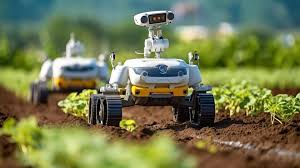
\includegraphics[width=0.4\textwidth]{logo.jpg}
    
\includegraphics[width=0.4\textwidth]{facepe.png}\\[1cm]
    {\textbf{\inserttitle}}\\[0.5cm]
    {\insertauthor}\\[0.3cm]
    {\small \insertdate}
\end{frame}

% ==========================================================
% ==================== CONTEXTUALIZAÇÃO ====================
% ==========================================================

\begin{frame}{Sumário}
    \tableofcontents
\end{frame}


\section{Contextualização}
\begin{frame}{Contextualização}
\begin{itemize}
    \item O uso de tecnologia e sustentabilidade.
    \item Agricultura de precisão exige monitoramento contínuo de variáveis ambientais.
    \item Pequenos produtores enfrentam limitações de custo e tecnologia.
    \item Este projeto propõe soluções acessíveis para coleta, análise e interpretação de dados ambientais em tempo real.
\end{itemize}
\end{frame}

% ==========================================================
% ========================= DESAFIOS =======================
% ==========================================================
\section{Desafios do projeto}
\begin{frame}{Desafios do Projeto}
\begin{tcolorbox}[colback=blue!5!white, colframe=blue!60!black, title=Principais Desafios, width=1.02\textwidth, enlarge left by=0mm, enlarge right by=0mm]
\centering
% Redimensiona todo o fluxograma para caber na caixa
\resizebox{1.0\textwidth}{!}{%
\begin{tikzpicture}[node distance=1cm, auto, >=stealth']

% Primeira coluna: Materiais
\node (materiais) [process] {Materiais e Sensores};
\node (materiais1) [io, below=0.5cm of materiais] {Limitação de kits e placas};
\node (materiais2) [io, below=0.5cm of materiais1] {Reutilização de componentes};
\node (materiais3) [io, below=0.5cm of materiais2] {Custos e disponibilidade};

% Segunda coluna: Aprendizagem
\node (aprendizagem) [process, right=4cm of materiais] {Aprendizagem Técnica};
\node (aprendizagem1) [io, below=0.5cm of aprendizagem] {Programação Arduino e Python};
\node (aprendizagem2) [io, below=0.5cm of aprendizagem1] {Eletrônica básica e circuitos};
\node (aprendizagem3) [io, below=0.5cm of aprendizagem2] {Integração hardware/software};

% Terceira coluna: Horários
\node (horarios) [process, right=4cm of aprendizagem] {Horários e Logística};
\node (horarios1) [io, below=0.5cm of horarios] {Limitação pelo horário escolar};
\node (horarios2) [io, below=0.5cm of horarios1] {Encontros extracurriculares};
\node (horarios3) [io, below=0.5cm of horarios2] {Coordenação das atividades};

% Conexões internas Materiais
\draw [arrow] (materiais.south) -- (materiais1.north);
\draw [arrow] (materiais1.south) -- (materiais2.north);
\draw [arrow] (materiais2.south) -- (materiais3.north);

% Conexões internas Aprendizagem
\draw [arrow] (aprendizagem.south) -- (aprendizagem1.north);
\draw [arrow] (aprendizagem1.south) -- (aprendizagem2.north);
\draw [arrow] (aprendizagem2.south) -- (aprendizagem3.north);

% Conexões internas Horários
\draw [arrow] (horarios.south) -- (horarios1.north);
\draw [arrow] (horarios1.south) -- (horarios2.north);
\draw [arrow] (horarios2.south) -- (horarios3.north);

\end{tikzpicture}%
}
\end{tcolorbox}
\end{frame}


% ==========================================================
% ==================== OBJETIVOS ===========================
% ==========================================================

\section{Objetivos}
\begin{frame}{Objetivos}
\begin{itemize}
    \item Desenvolver um sistema de baixo custo para monitoramento ambiental agrícola.
    \item Capacitar estudantes e bolsistas na integração entre eletrônica, programação e análise de dados.
    \item Promover práticas de agricultura sustentável, apoiadas em evidências estatísticas.
\end{itemize}
\end{frame}

% ==========================================================
% ====================== JUSTIFICATIVA ======================
% ==========================================================
\section{Justificativas}
\begin{frame}{Justificativas}
\begin{itemize}

    \item \textbf{Dados precisos reduzem desperdícios:}
    \begin{itemize}
        \item Evitam irrigação excessiva;
        \item Reduzem uso de água, energia e insumos;
        \item Aumentam a eficiência no manejo agrícola;
        \item Permitem decisões baseadas em evidências.
    \end{itemize}

    \item \textbf{Integração entre tecnologia e sustentabilidade:}
    \begin{itemize}
        \item Uso de sensores de baixo custo e análise de dados;
        \item Promoção da agricultura inteligente e acessível;
        \item Redução do impacto ambiental nas práticas agrícolas;
        \item Incentivo à produção mais responsável e eficiente.
    \end{itemize}

\end{itemize}
\end{frame}


% ==========================================================
% ==================== MÉTODOS =============================
% ==========================================================

\section{Métodos}
\begin{frame}{Métodos}
\begin{itemize}
    \item Coleta automatizada de dados utilizando \textbf{Arduino Uno/Nano} com os sensores:
    \begin{itemize}
        \item \textbf{DHT11} – temperatura e umidade do ar;
        \item \textbf{HD-38} – umidade do solo.
    \end{itemize}

    \item Armazenamento das medições em \textbf{cartão SD} para registro contínuo.

    \item Processamento e análise dos dados em \textbf{Python}, utilizando:
    \begin{itemize}
        \item \textit{Pandas} –cálculos estatísticos;
        \item \textit{NumPy} – recursos para cálculos;
        \item \textit{Matplotlib} e \textit{Seaborn} – visualização gráfica.
    \end{itemize}
\end{itemize}
\end{frame}


\begin{frame}{Fluxograma do Sistema}
\centering
\resizebox{1.06\textwidth}{!}{%
\begin{tikzpicture}[
  node distance=14mm and 25mm,
  font=\small,
  startstop/.style={ellipse, draw, fill=gray!25, minimum width=40mm, minimum height=10mm, align=center},
  process/.style={rectangle, draw, fill=blue!20, rounded corners, minimum width=50mm, minimum height=10mm, align=center},
  io/.style={trapezium, trapezium left angle=70, trapezium right angle=110, draw, fill=green!20, minimum width=50mm, minimum height=10mm, align=center},
  python/.style={rectangle, draw, fill=orange!25, rounded corners, minimum width=55mm, minimum height=10mm, align=center},
  arrow/.style={thick, -{Stealth[length=3mm]}}
]

% Nodes
\node[startstop] (inicio) {Início do Sistema};
\node[process, below=of inicio] (leitura) {Leitura dos Sensores \\ (DHT11: Temp. e Umidade do Ar, HD-38: Umidade do Solo)};
\node[process, below=of leitura] (estatistica) {Geração de Estatísticas (média, mediana, desvio-padrão, intervalo interquartil) \\ e Gravação no Cartão SD};
\node[startstop, below=of estatistica, yshift=-2mm] (loop) {Loop Contínuo de Aquisição};

\node[python, right=30mm of estatistica] (python) {Leitura dos Dados com Python e Pandas \\ para análise e visualização};

% Arrows
\draw[arrow] (inicio) -- (leitura);
\draw[arrow] (leitura) -- (estatistica);
\draw[arrow] (estatistica) -- (loop);
\draw[arrow] (loop.east) -- ++(28mm,0) |- (leitura.east);
\draw[arrow, dashed] (estatistica.east) -- ++(25mm,0) -- (python.west);

% Annotation
\node[align=center, below=10mm of python, font=\footnotesize] {Fluxograma de aquisição e processamento de dados:  \\ o Arduino executa o loop contínuo de leitura e armazenamento, \\ enquanto a análise com Python ocorre externamente.};

\end{tikzpicture}
} % resizebox
\vspace{2mm}
{\tiny \textbf{Fonte:} Autor (2025).}
\end{frame}
\end{frame}


% ==========================================================
% ==================== RESULTADOS =========================
% ==========================================================

\section{Resultados}
\begin{frame}{Resultados — Temperatura do Ar}
\begin{itemize}
    \item Intervalo: \textbf{1,4°C} (de 24,8°C a 26,2°C);
    \item Média: \textbf{25,45°C};
    \item Mediana: \textbf{25,4°C};
    \item Desvio padrão: \textbf{0,42°C}.
\end{itemize}

\begin{figure}[h]
    \centering
    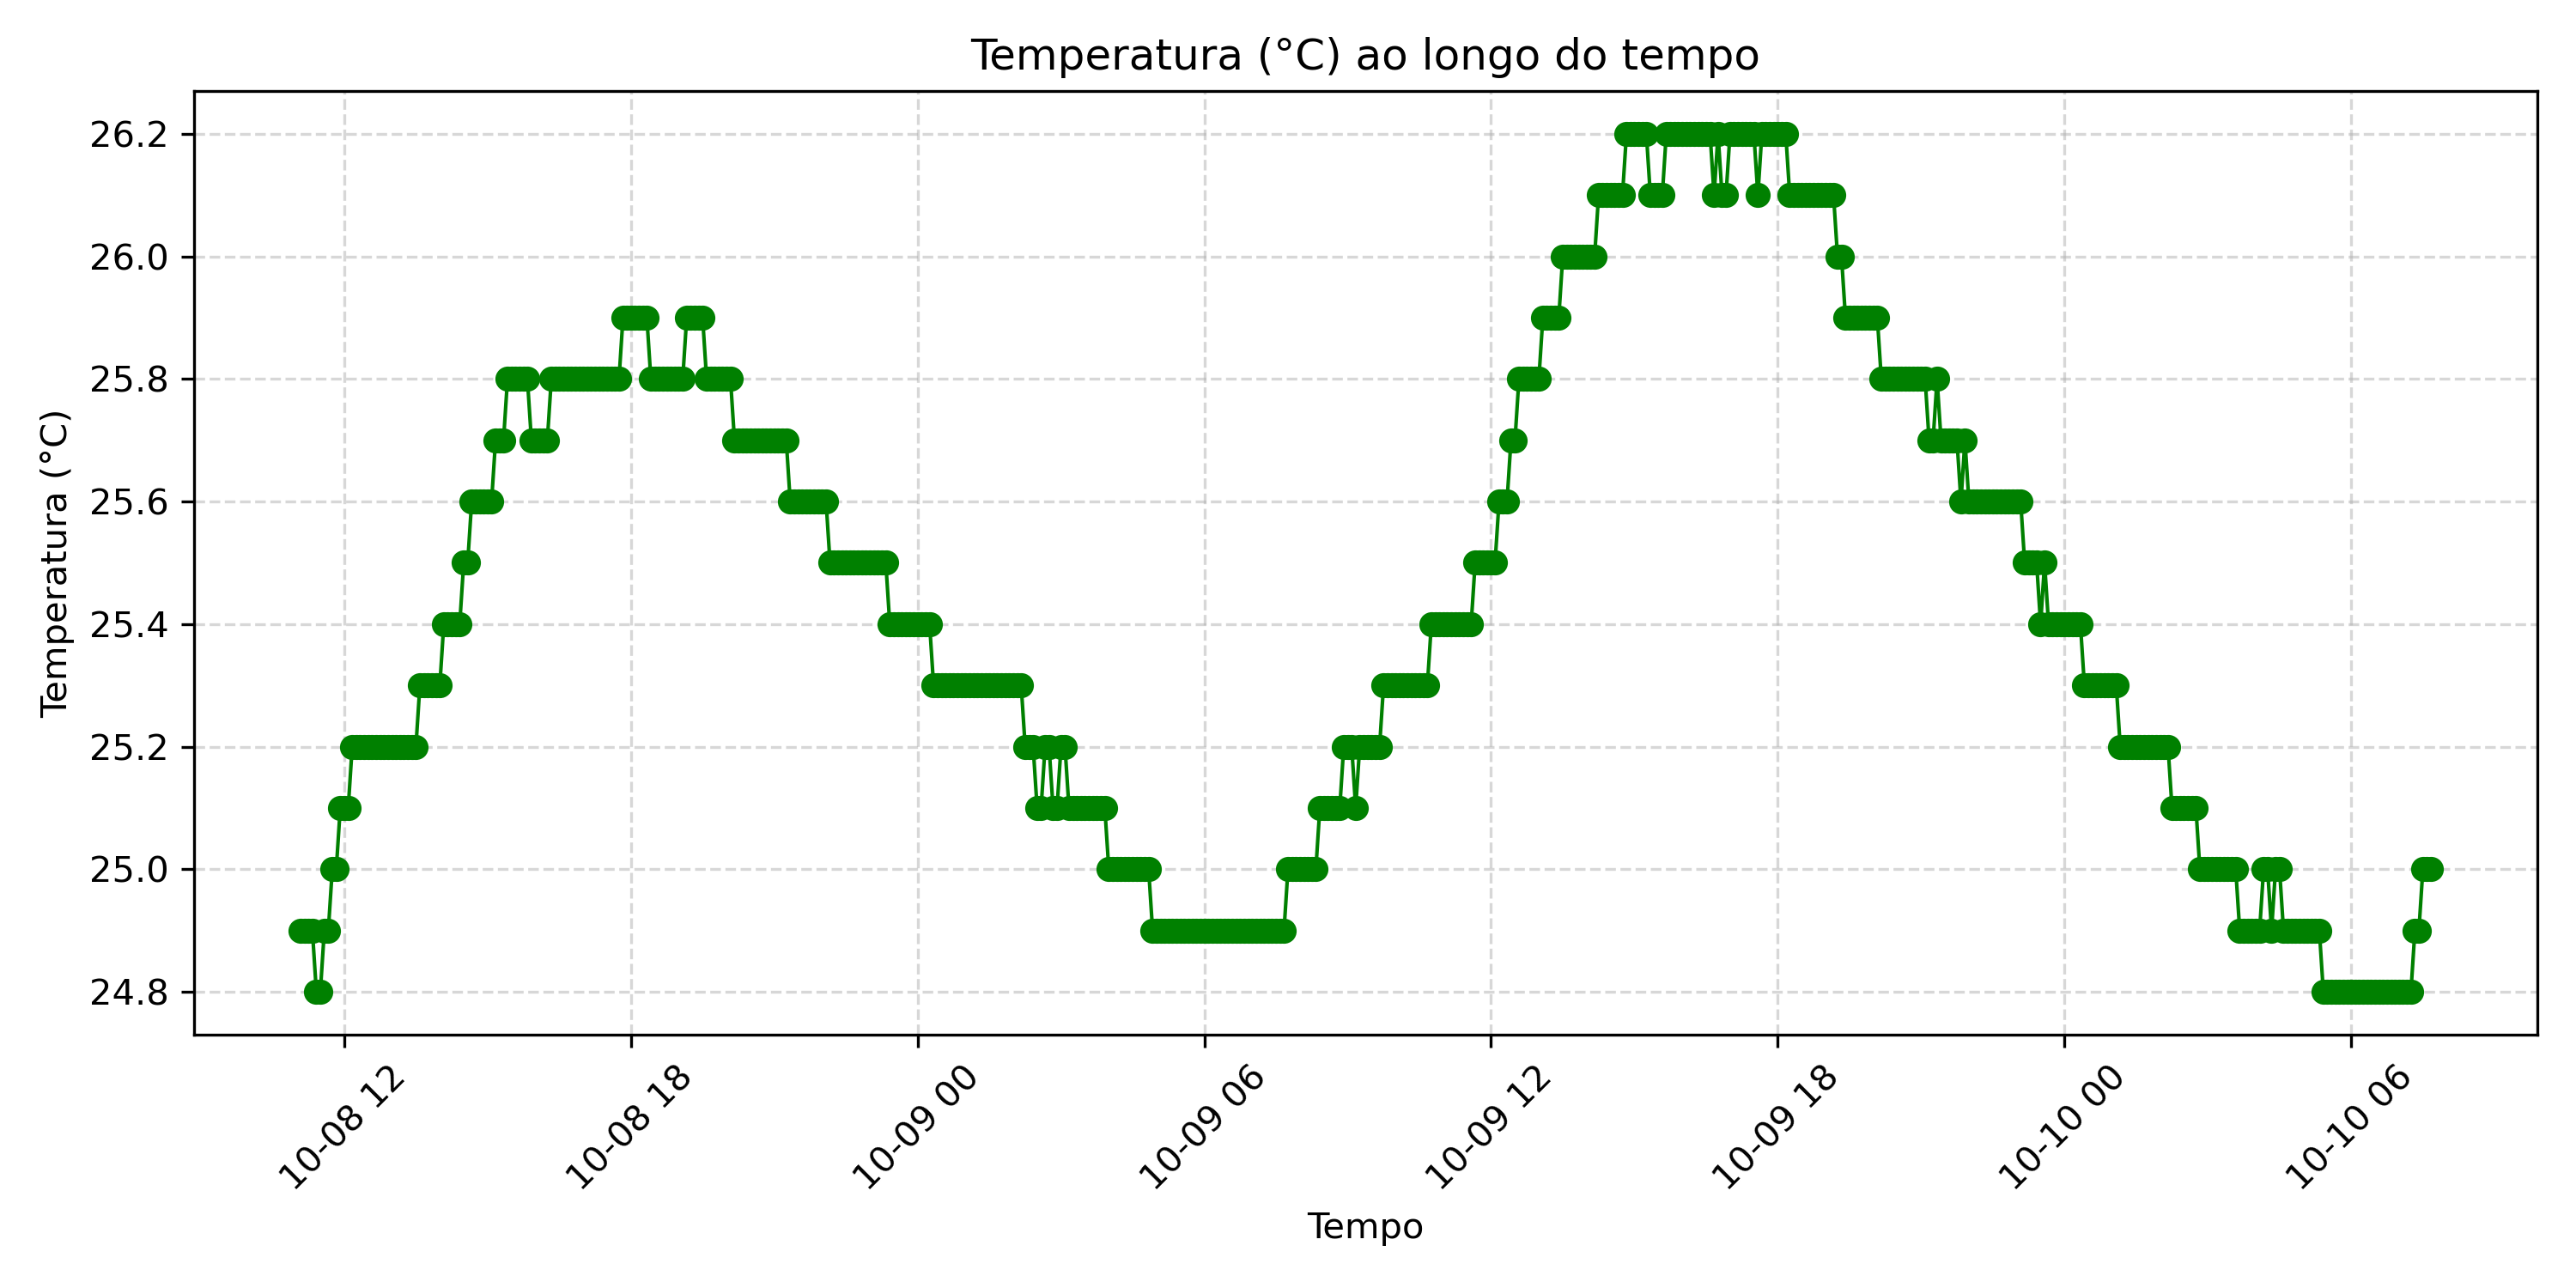
\includegraphics[width=0.6\textwidth]{Temp.png}
    \caption{Variação temporal da temperatura do ar}
\end{figure}
    \vspace{-0.5cm}

\textbf{Conclusão:} Temperatura estável e homogênea, adequada a culturas tropicais.
\end{frame}

\begin{frame}{Resultados — Umidade do Ar}
\begin{itemize}
    \item Intervalo: \textbf{10,0\%};
    \item Média: \textbf{46,92\%};
    \item Mediana: \textbf{47,0\%};
    \item Desvio padrão: \textbf{1,70\%}.
\end{itemize}

\begin{figure}[h]
    \centering
    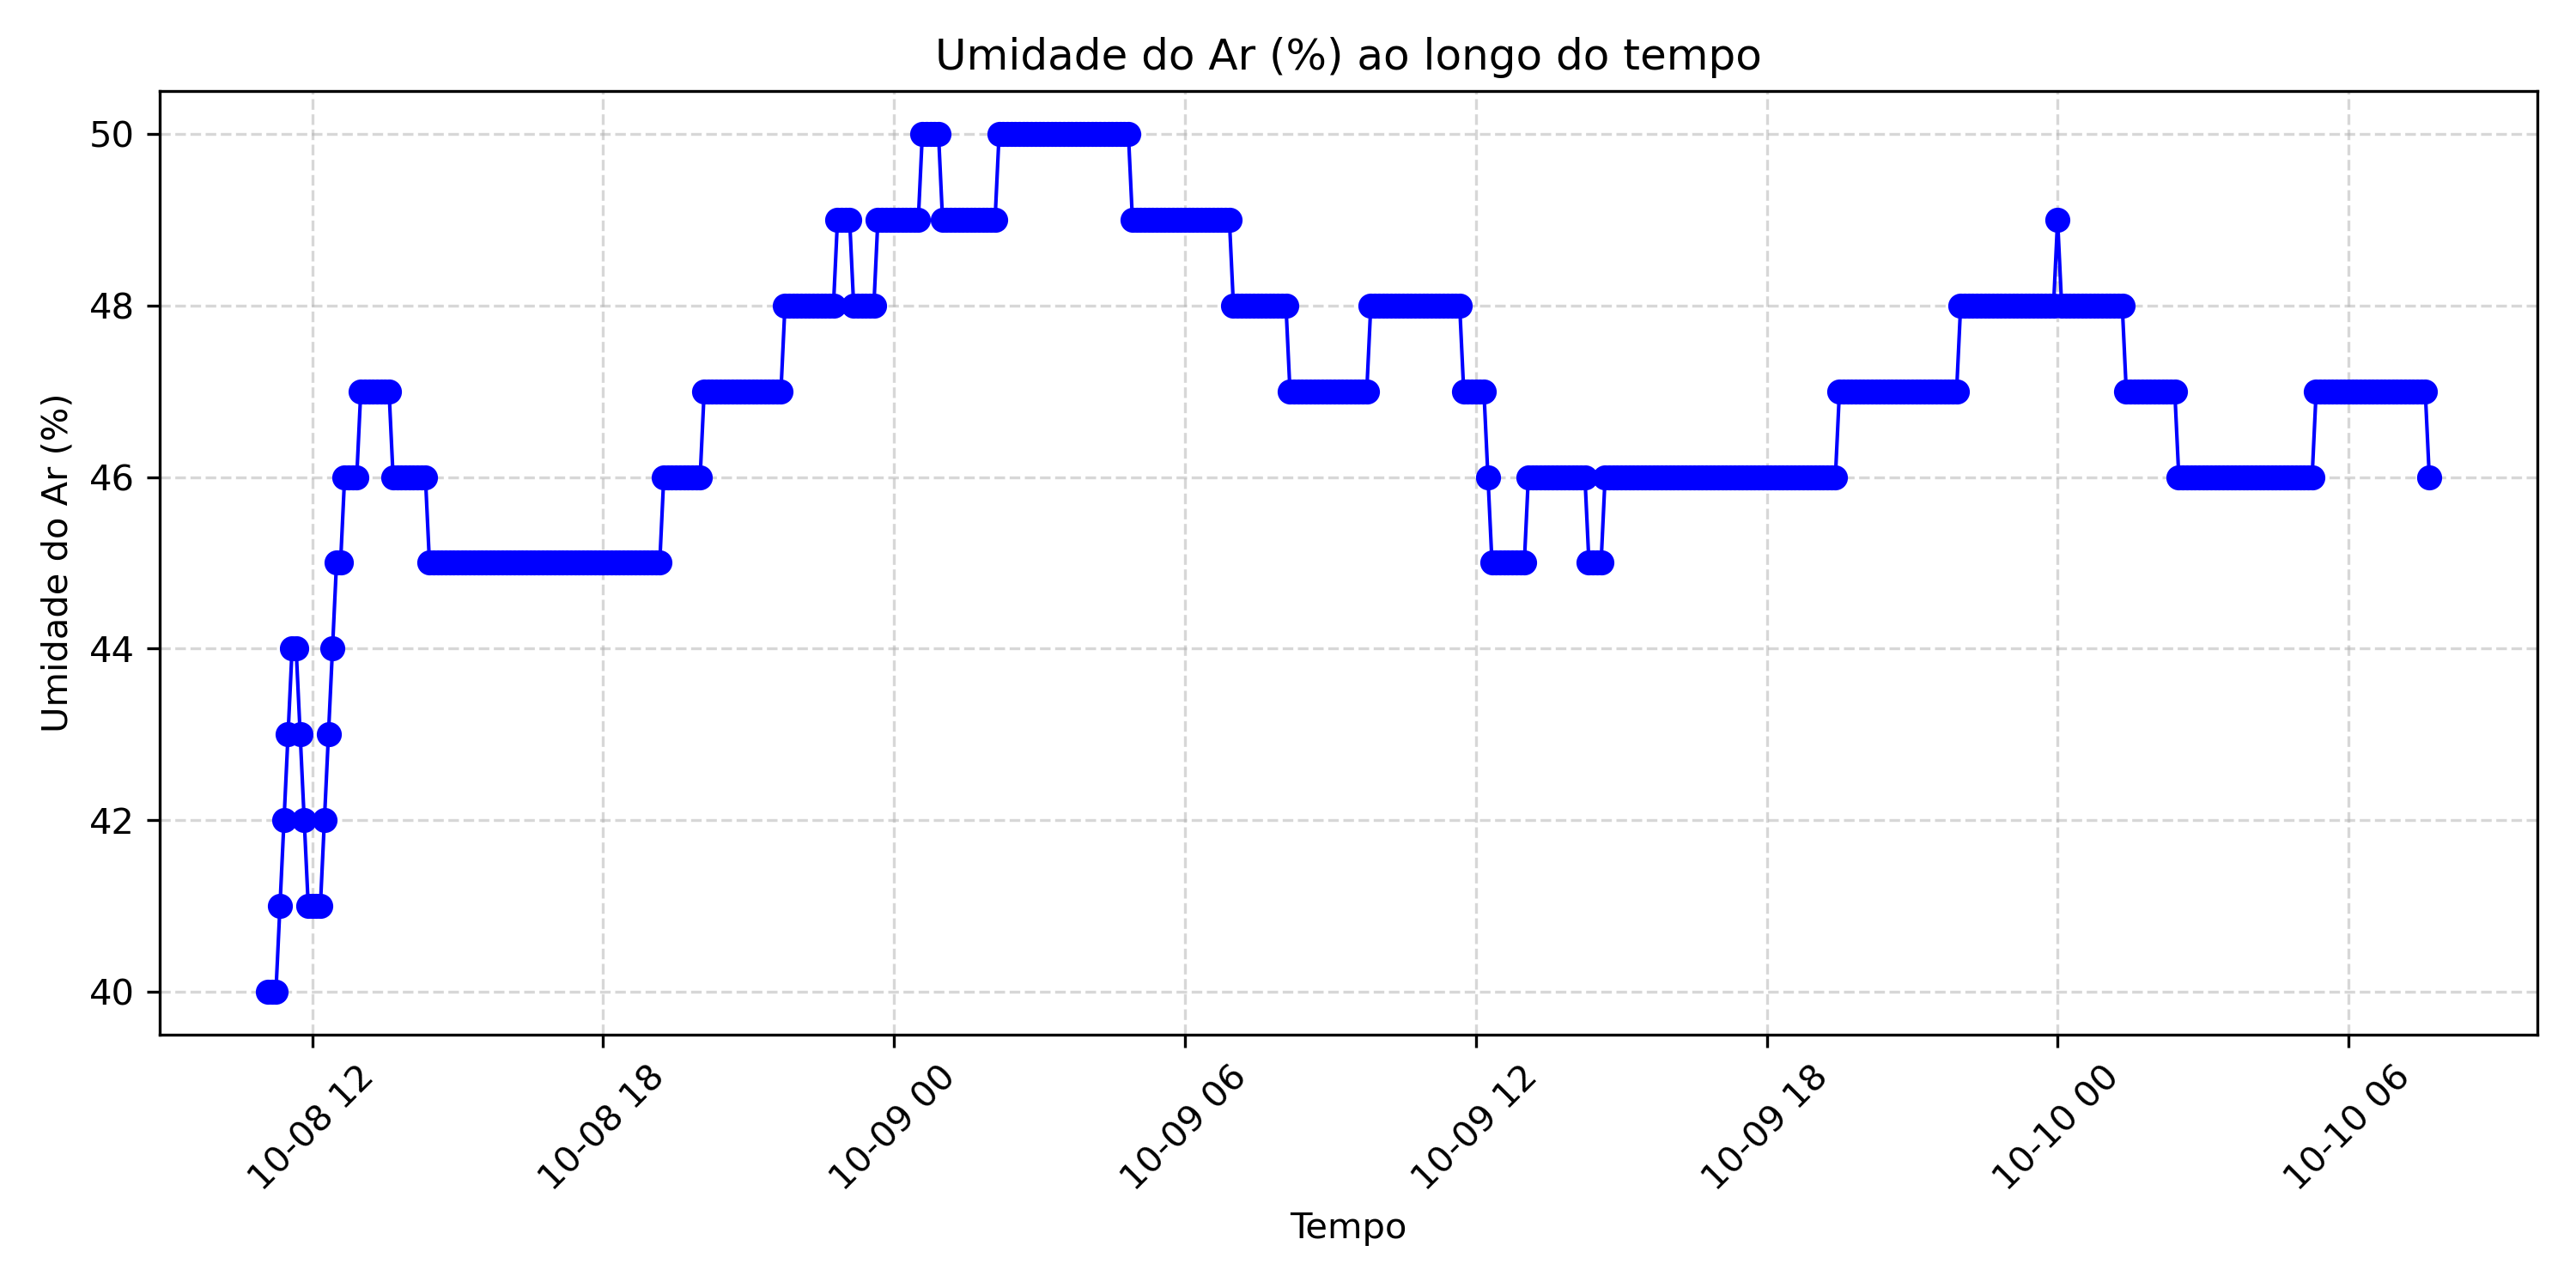
\includegraphics[width=0.6\textwidth]{UmidadeAr.png}
    \caption{Variação da umidade relativa do ar}
\end{figure}
    \vspace{-0.5cm}

\textbf{Conclusão:} Umidade do ar estável, ideal para hortaliças delicadas.
\end{frame}

\begin{frame}{Resultados — Umidade do Solo}
\begin{itemize}
    \item Intervalo: \textbf{31,0\%};
    \item Média: \textbf{80,39\%};
    \item Mediana: \textbf{82,0\%};
    \item Desvio padrão: \textbf{4,78\%}.
\end{itemize}

\begin{figure}[h]
    \centering
    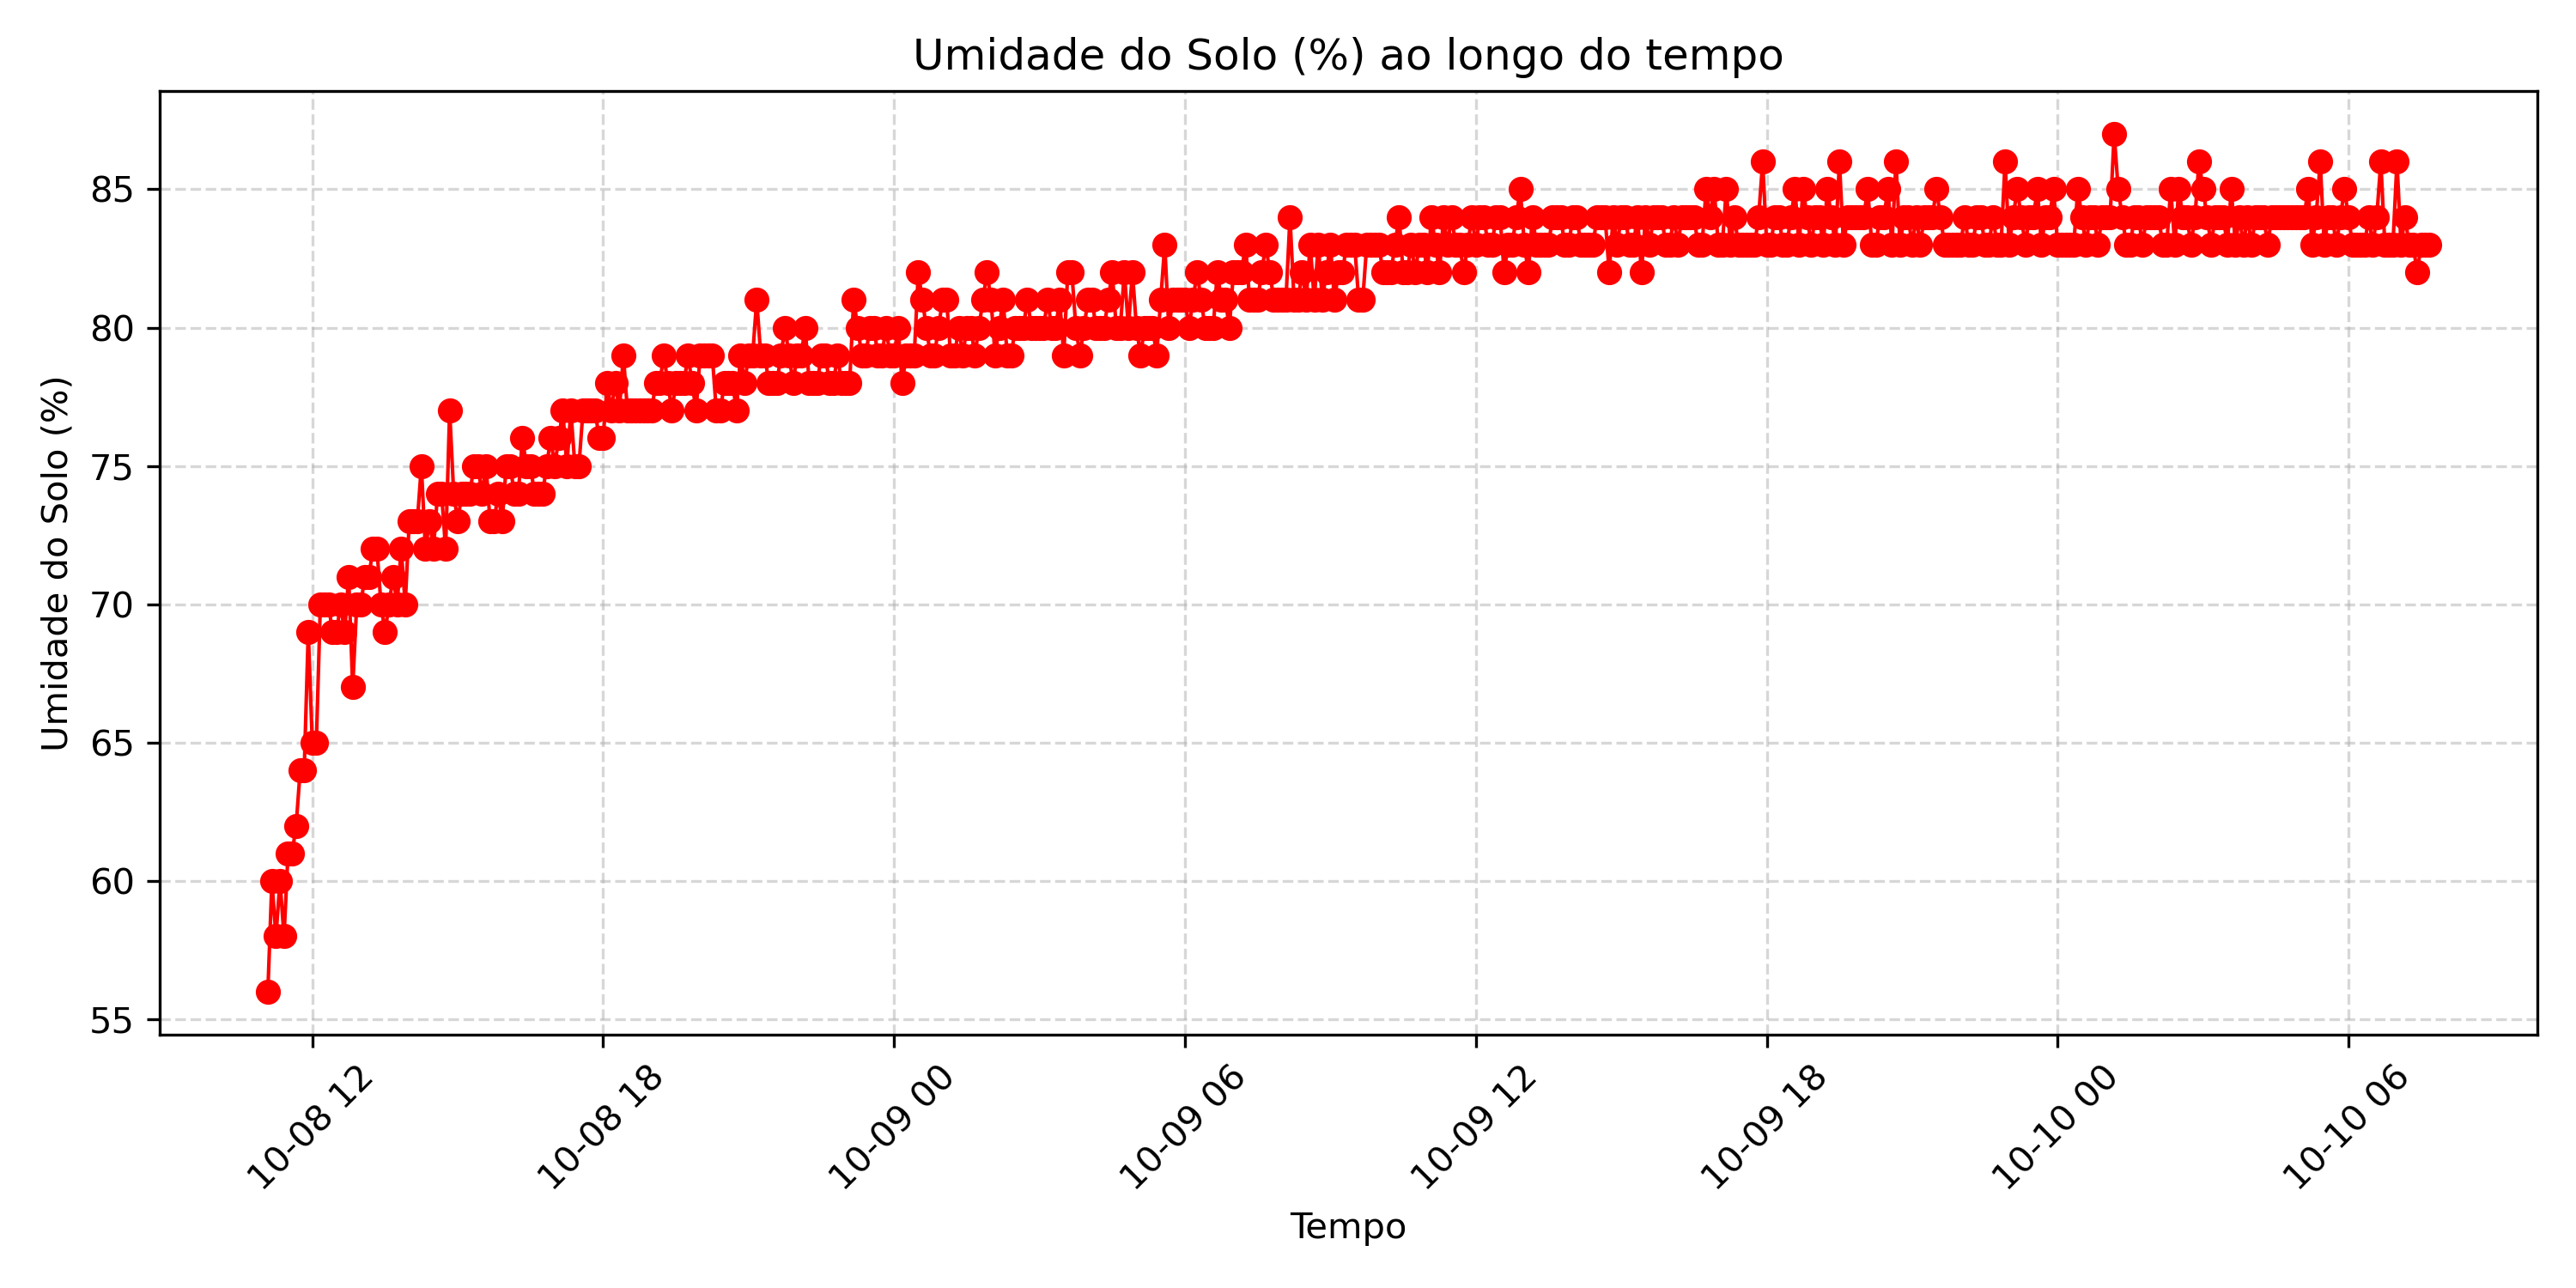
\includegraphics[width=0.6\textwidth]{USolo.png}
    \caption{Variação da umidade do solo}
\end{figure}
    \vspace{-0.5cm}
\textbf{Conclusão:} Solo com alta retenção hídrica, ideal para raízes e tubérculos.
\end{frame}

% ==========================================================
% ==================== ENTREGA E EVIDÊNCIAS ==============
% ==========================================================

\section{Entregáveis}
\begin{frame}{Entregáveis}
\begin{itemize}
    \item Sistema funcional para monitoramento ambiental.
    \item Dados coletados e analisados com gráficos e correlações.
    \item Recomendações agrícolas baseadas em evidências objetivas.
\end{itemize}

\begin{figure}[h]
\centering

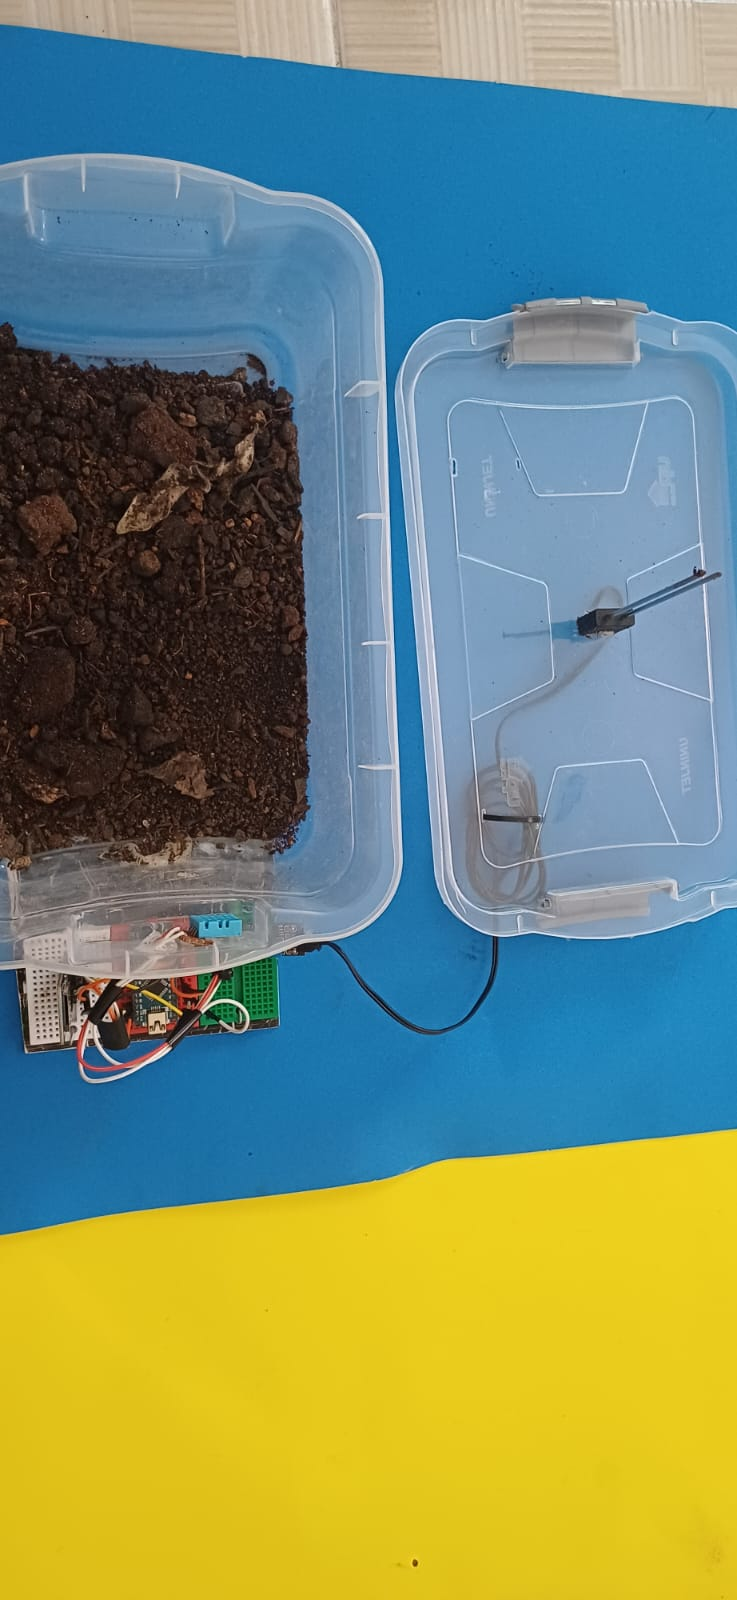
\includegraphics[
  width=0.28\textwidth,
  angle=90,
  trim={0cm 17cm 0cm 5cm},
  clip
]{AnalizadorSolo2.jpeg}
    \hspace{1mm}
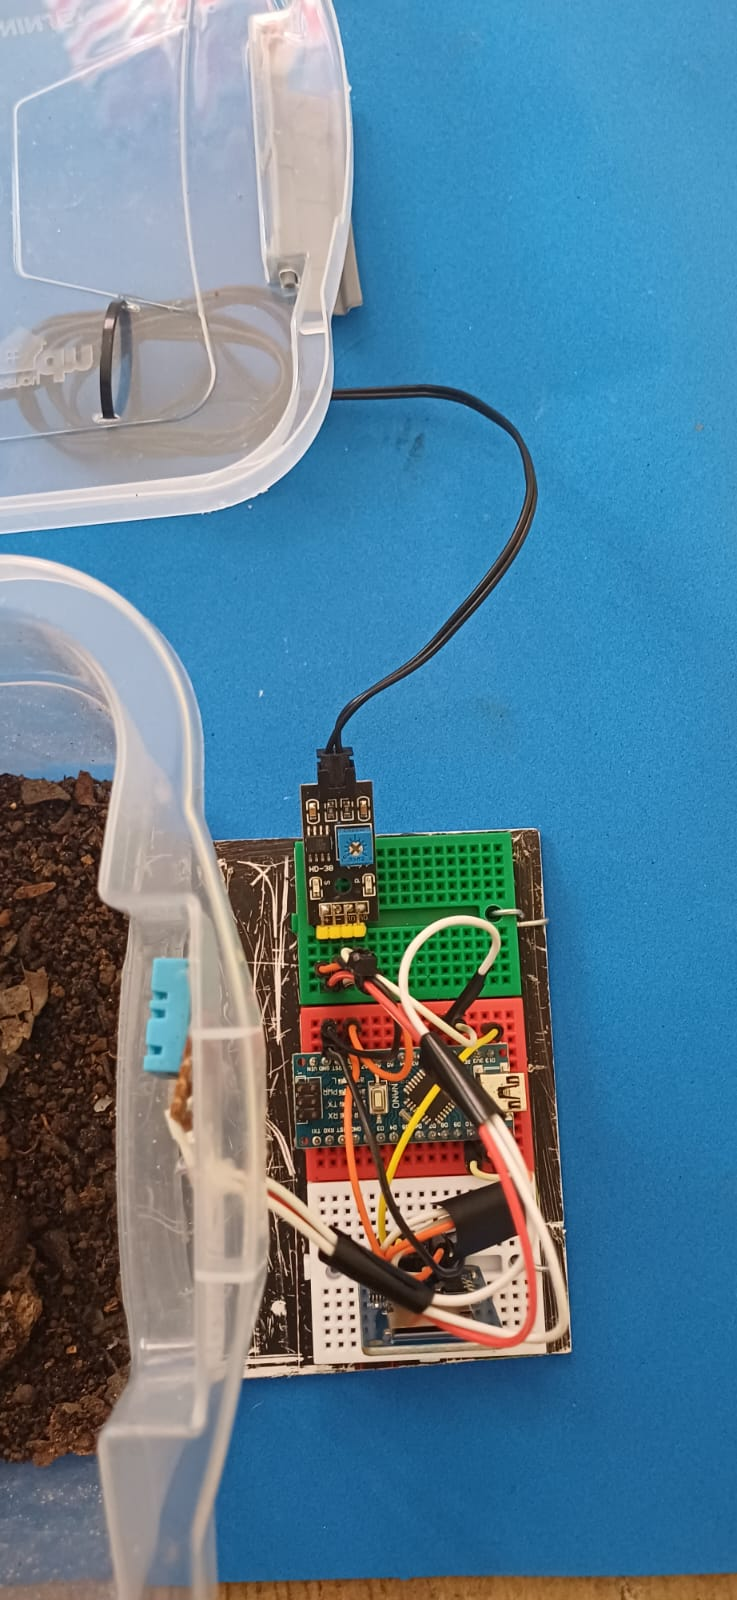
\includegraphics[
  width=0.28\textwidth,
  angle=90,
  trim={0cm 0cm 0cm 5cm},
  clip
]{AnalizadorSolo3.jpeg}
        \caption{Analizador de solo}
\end{figure}
\end{frame}

% ==========================================================
% ==================== ENGAJAMENTO ========================
% ==========================================================

\section{Engajamento}
\begin{frame}{Engajamento}
\begin{itemize}
    \item Alunos participaram da montagem, programação e análise de dados.
    \item Parceria com empresa Berro Tech e participação da comunidade.
    \item Apresentação de projetos e resultados em Amostra Cientifica GRE Arcoverde.
\end{itemize}
\end{frame}

% ==========================================================
% ==================== EVIDÊNCIAS ==========================
% ==========================================================

\section{Evidências}
\begin{frame}{Evidências}
    \begin{figure}[h]
        \centering
        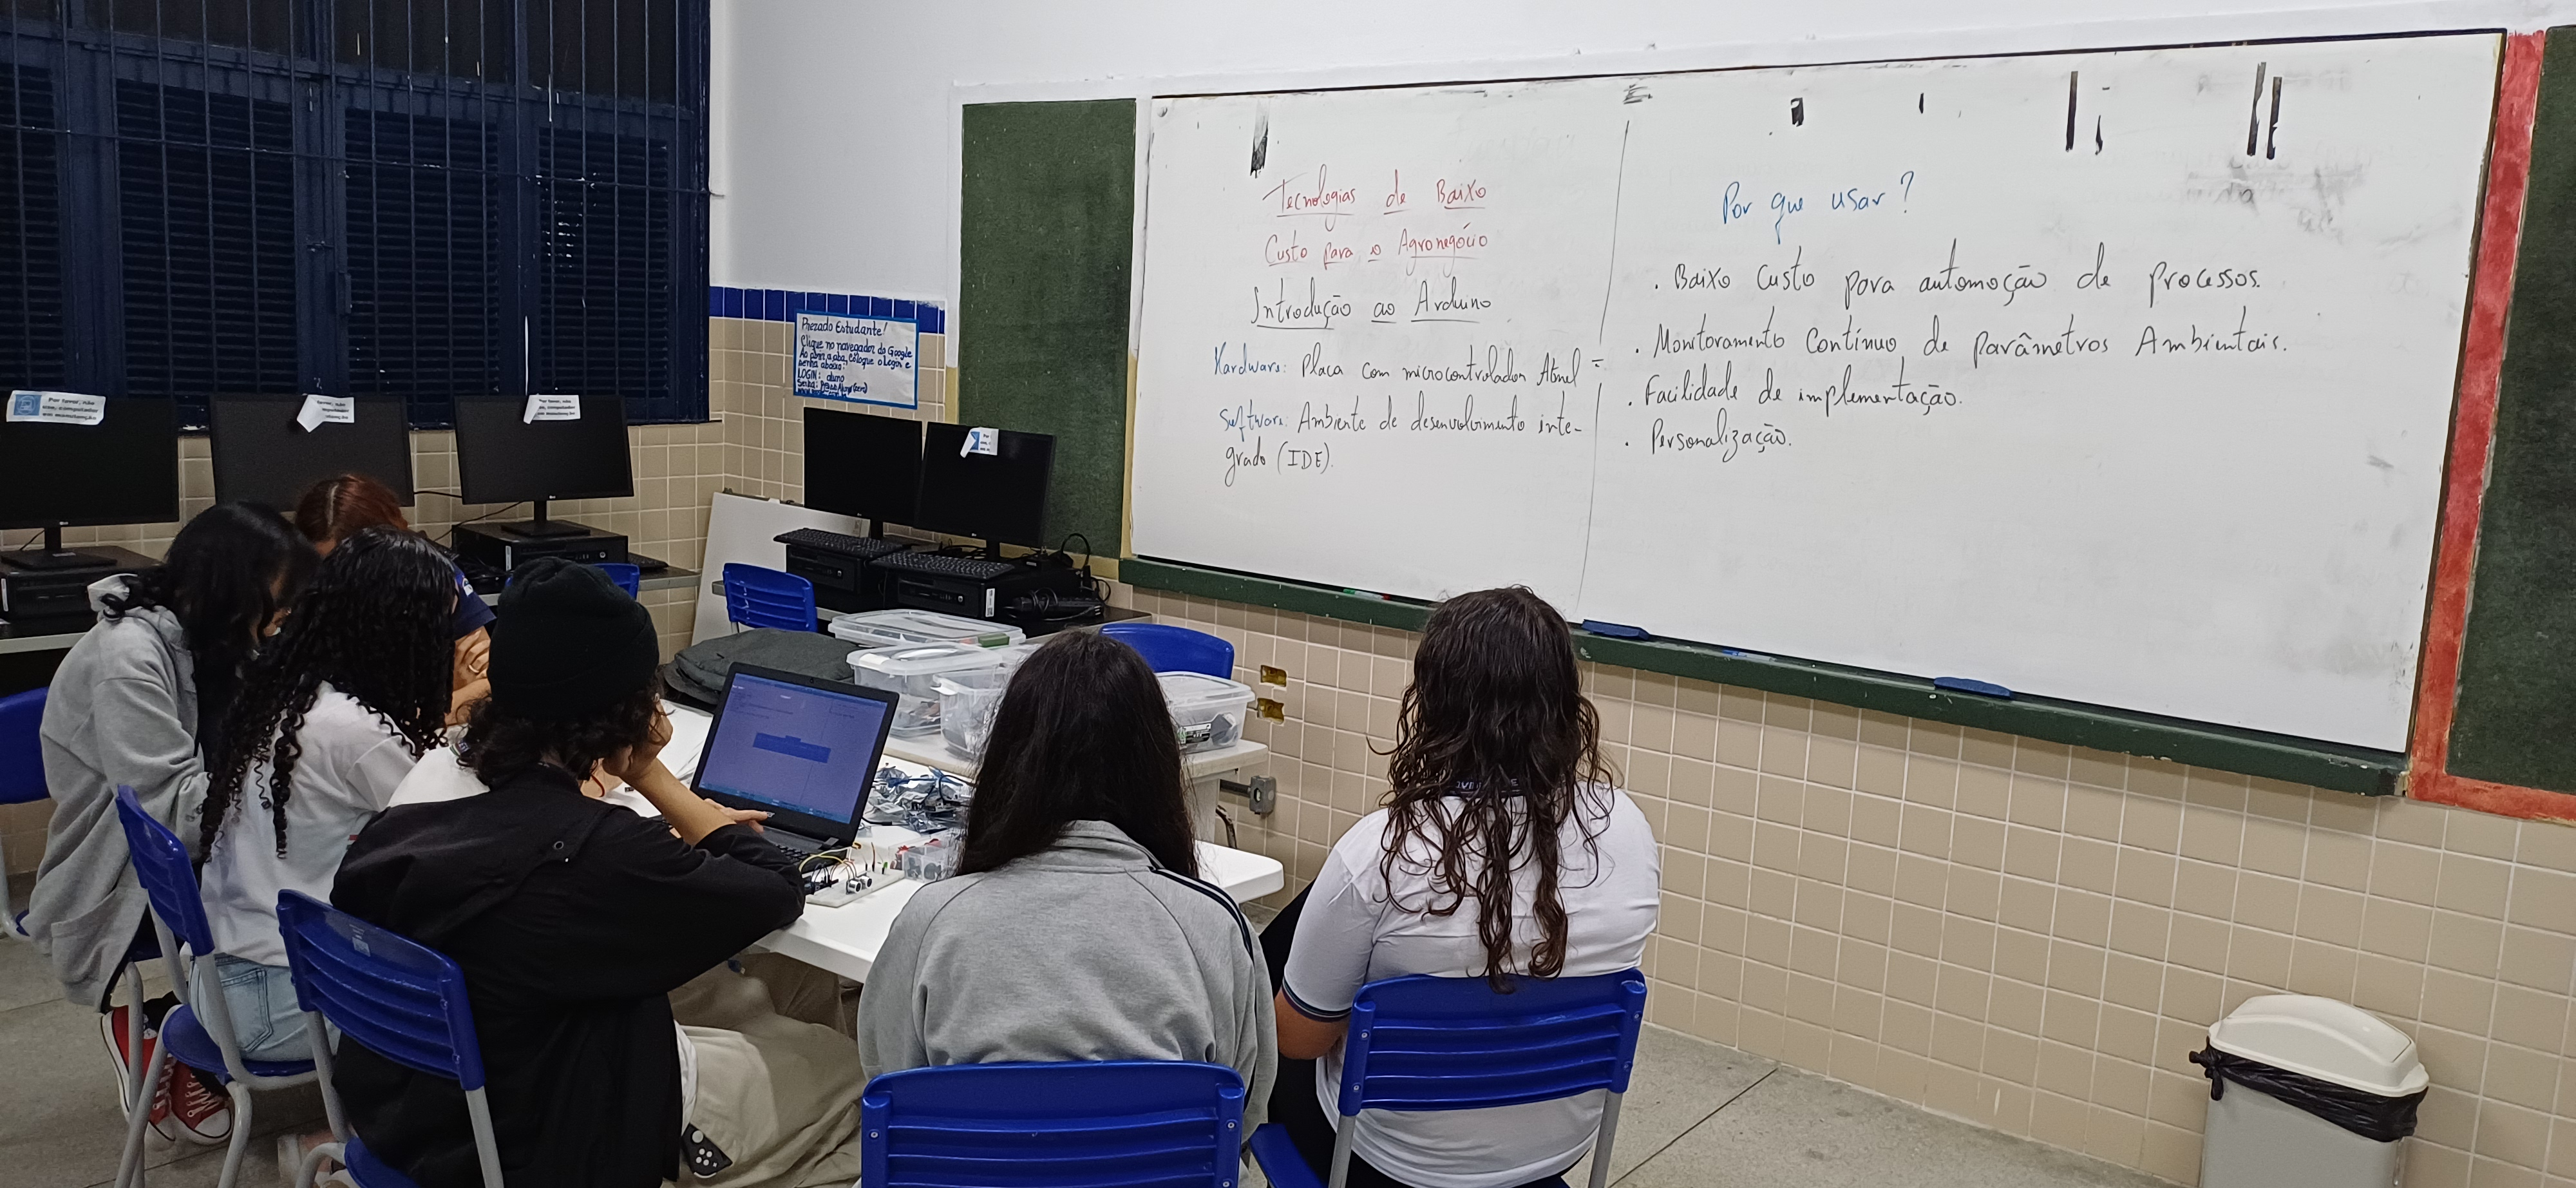
\includegraphics[width=0.4\textwidth]{../Fotos_Projeto_Arduino_Agronegocio/Etapa_1_Introducao/Ensino1.jpg}
        
\includegraphics[width=0.4\textwidth]{../Fotos_Projeto_Arduino_Agronegocio/Etapa_1_Introducao/galera5.jpg}
        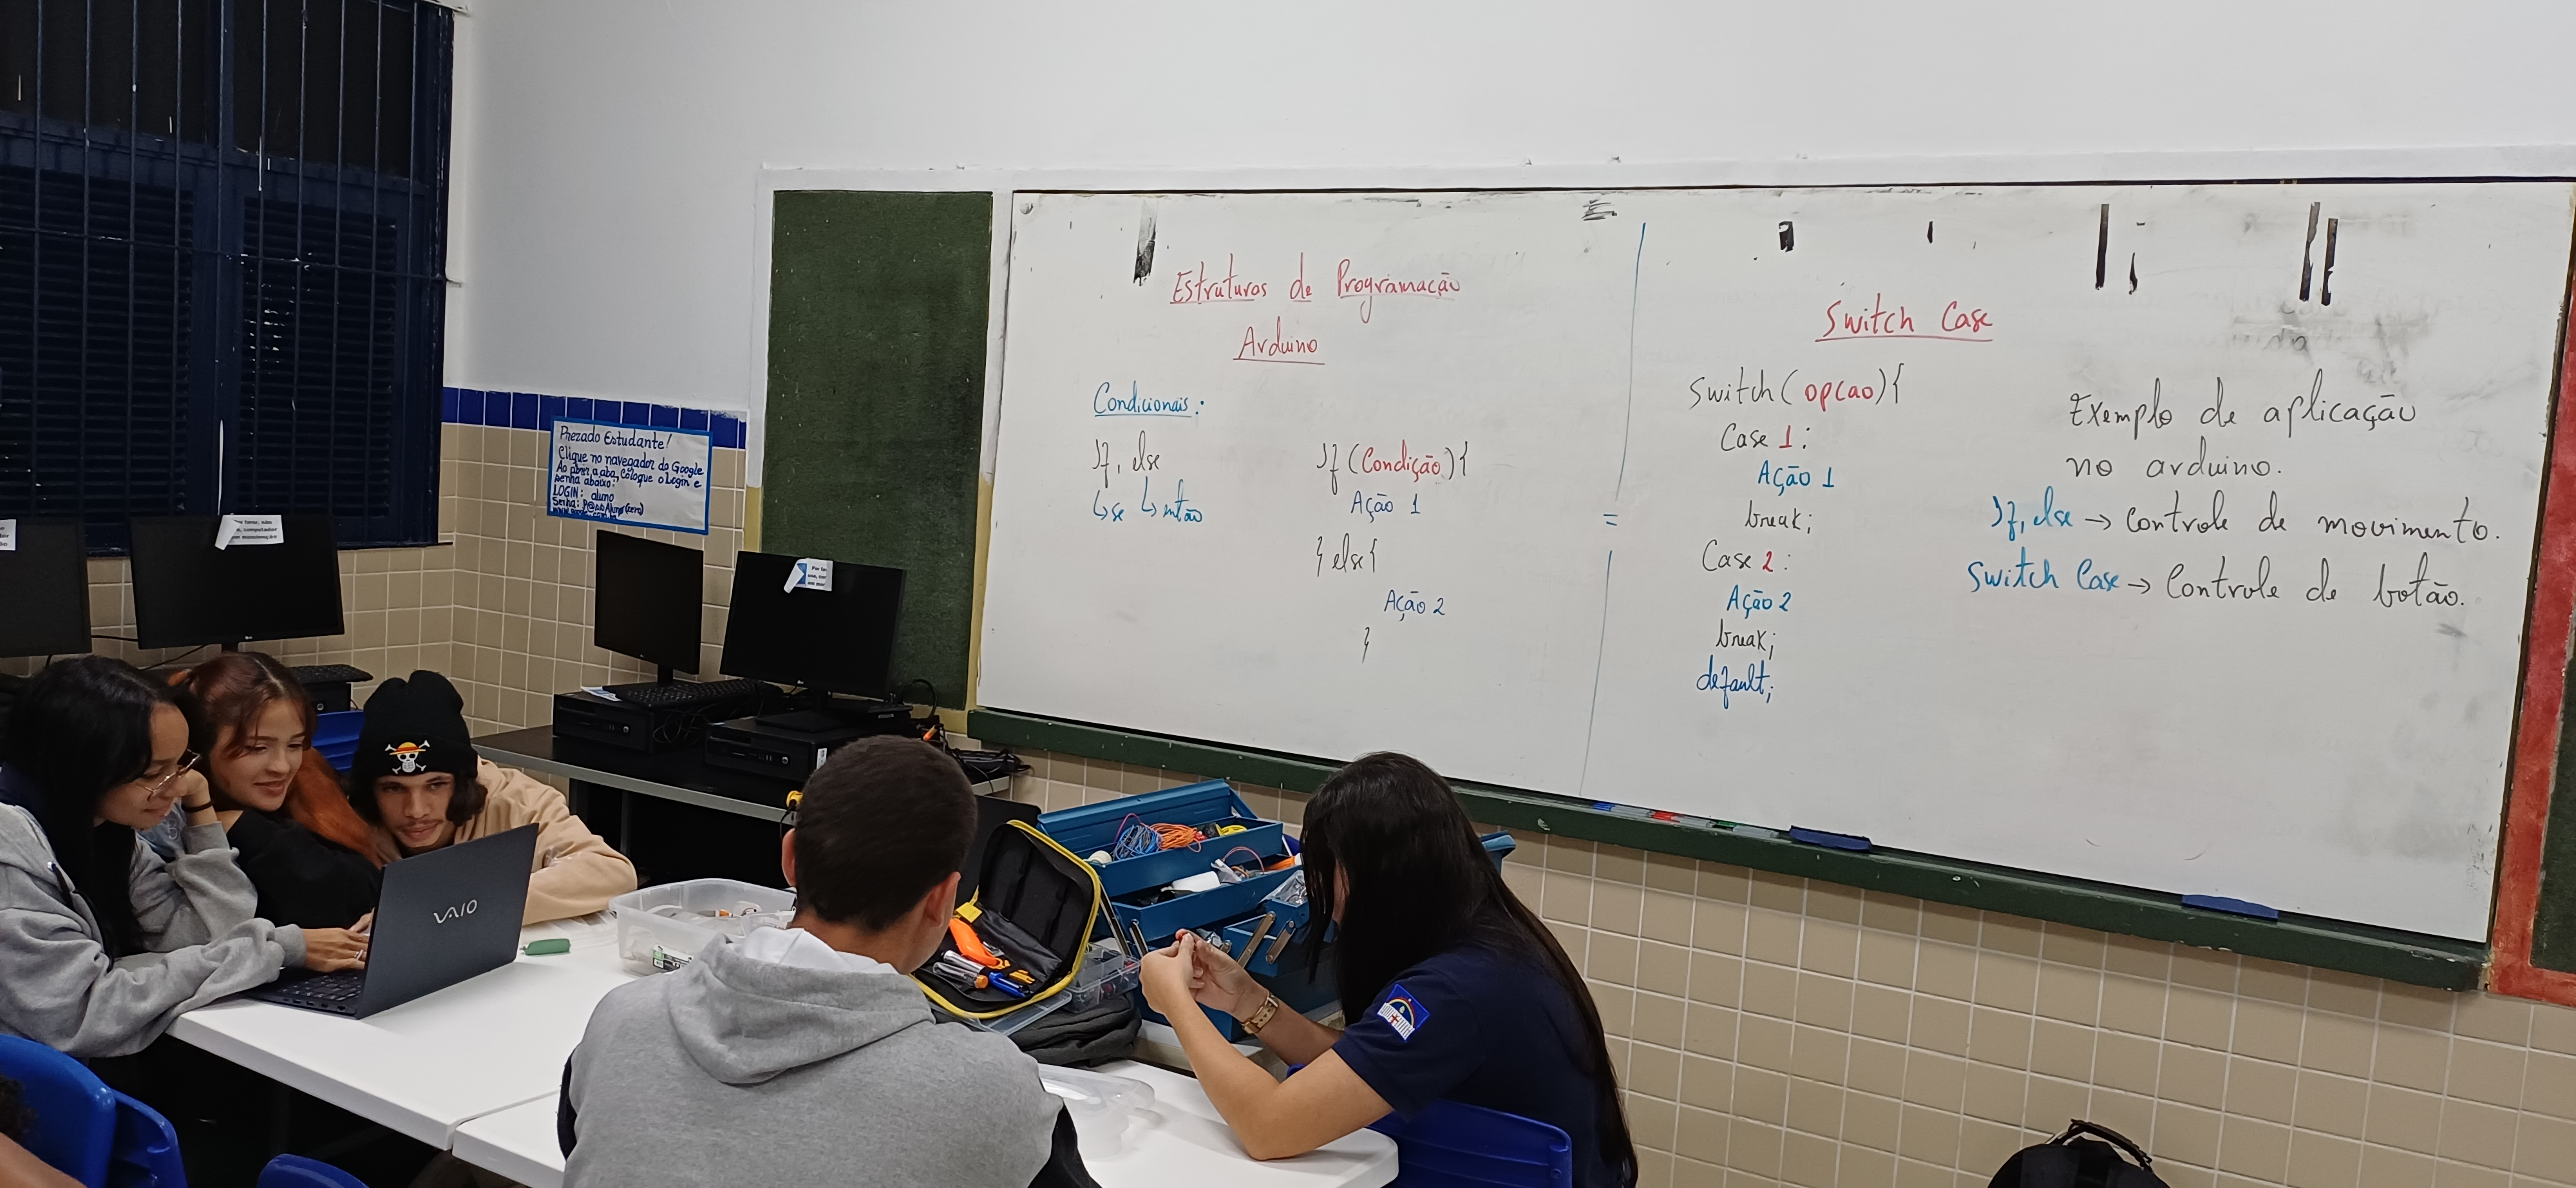
\includegraphics[width=0.4\textwidth]{../Fotos_Projeto_Arduino_Agronegocio/Etapa_3_Condicionais/20250820_203148.jpg}
        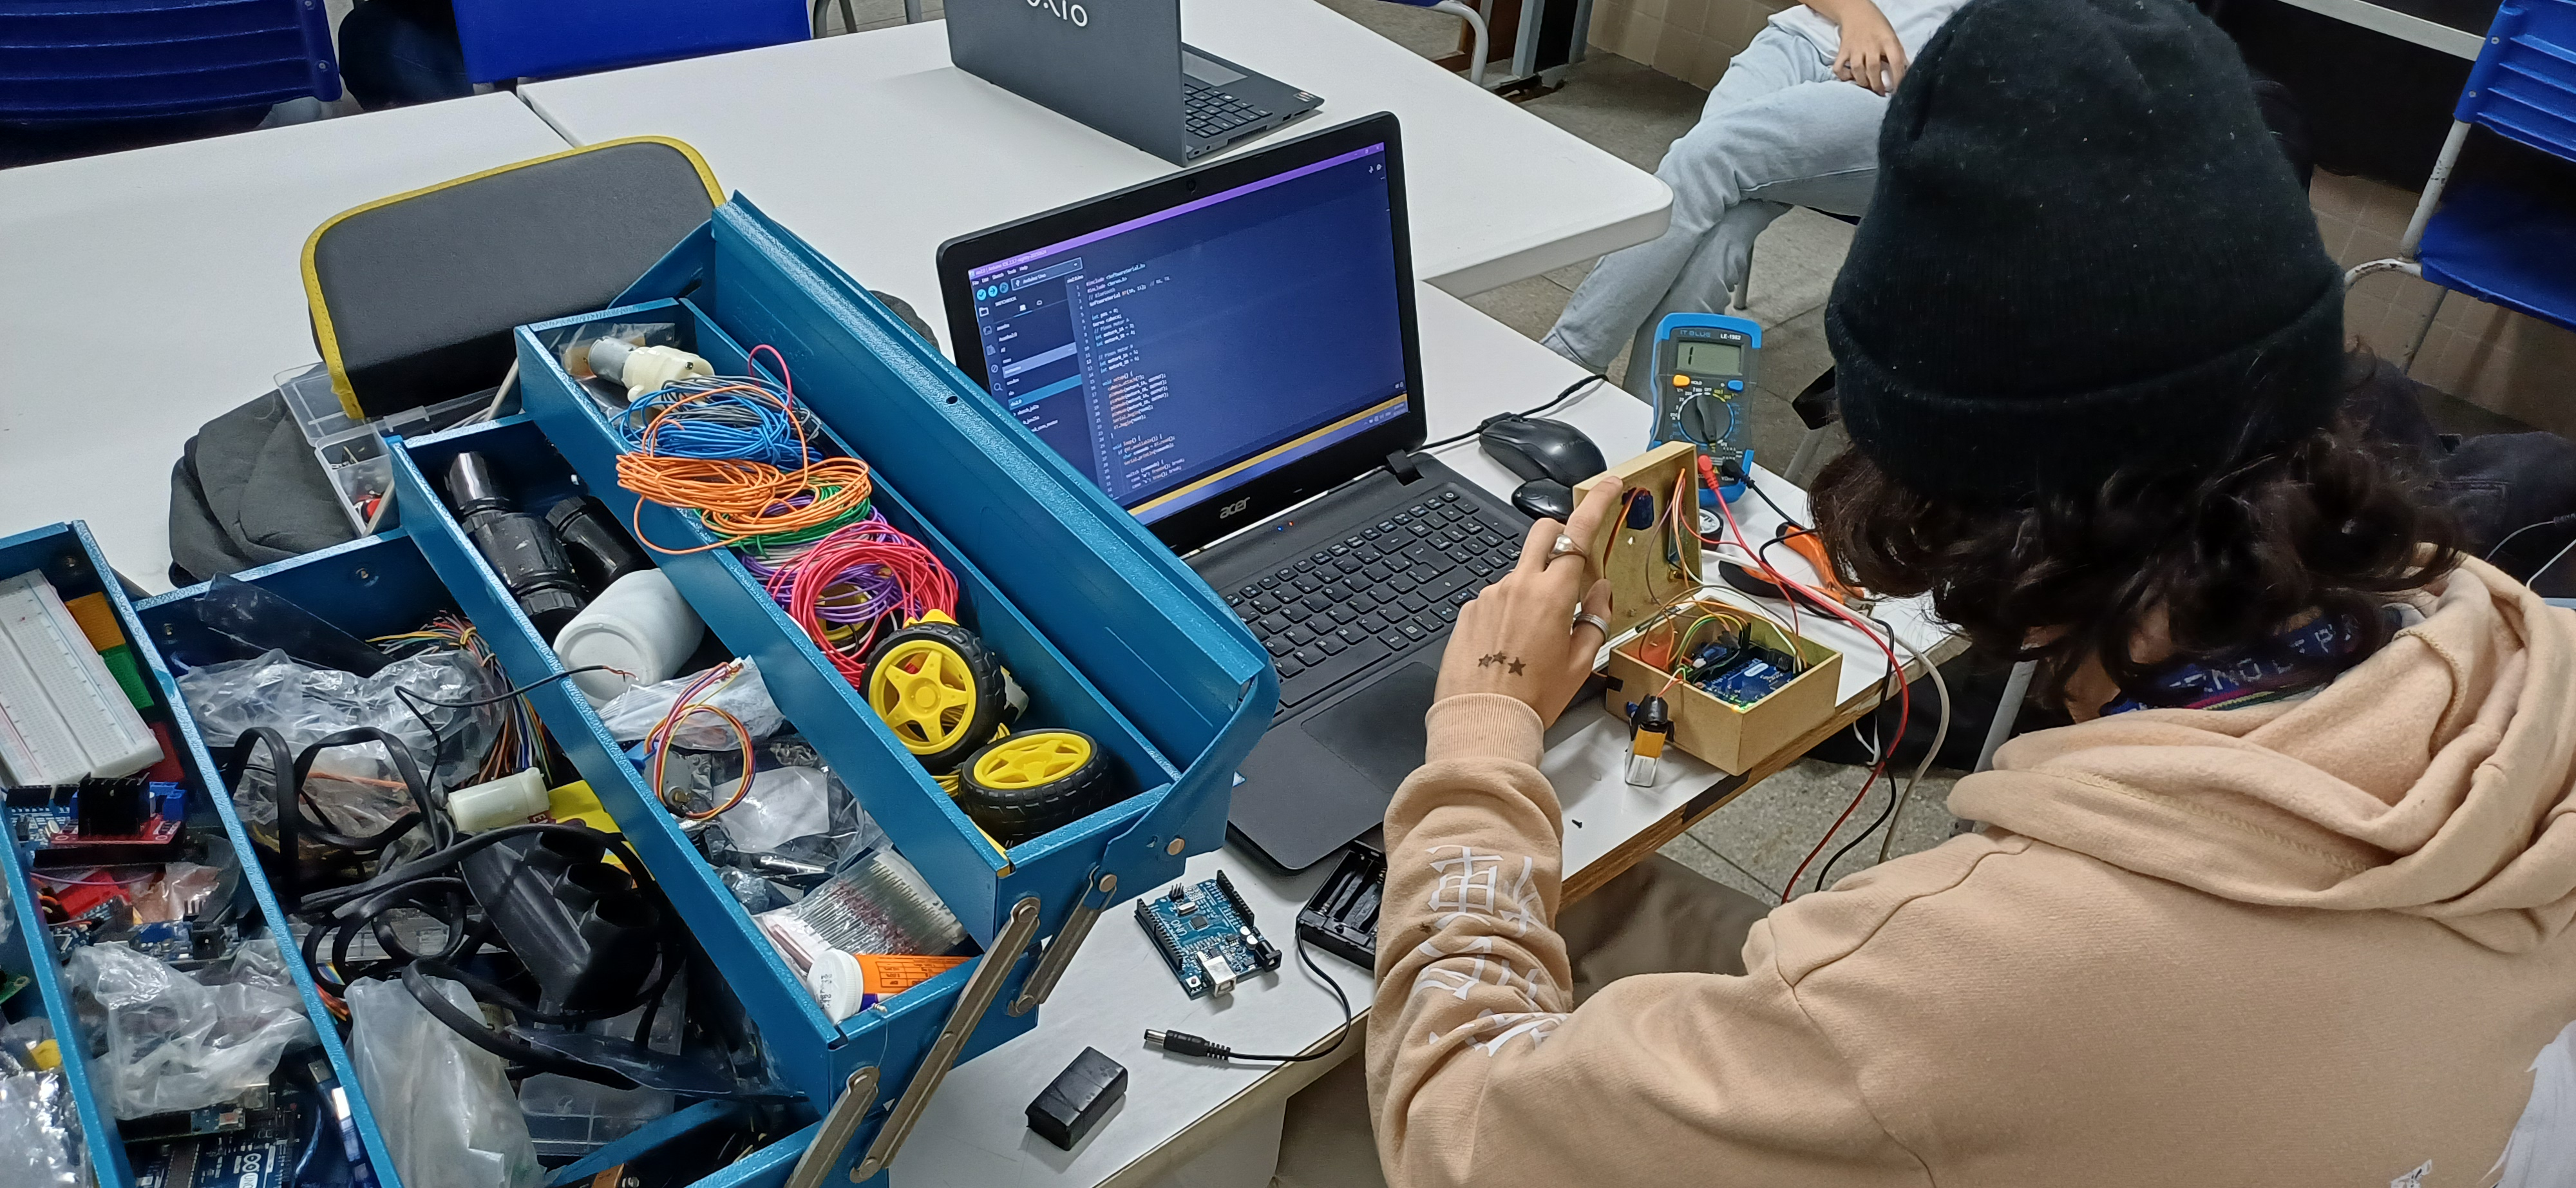
\includegraphics[width=0.4\textwidth]{../Fotos_Projeto_Arduino_Agronegocio/Etapa_3_Condicionais/20250820_203410.jpg}
        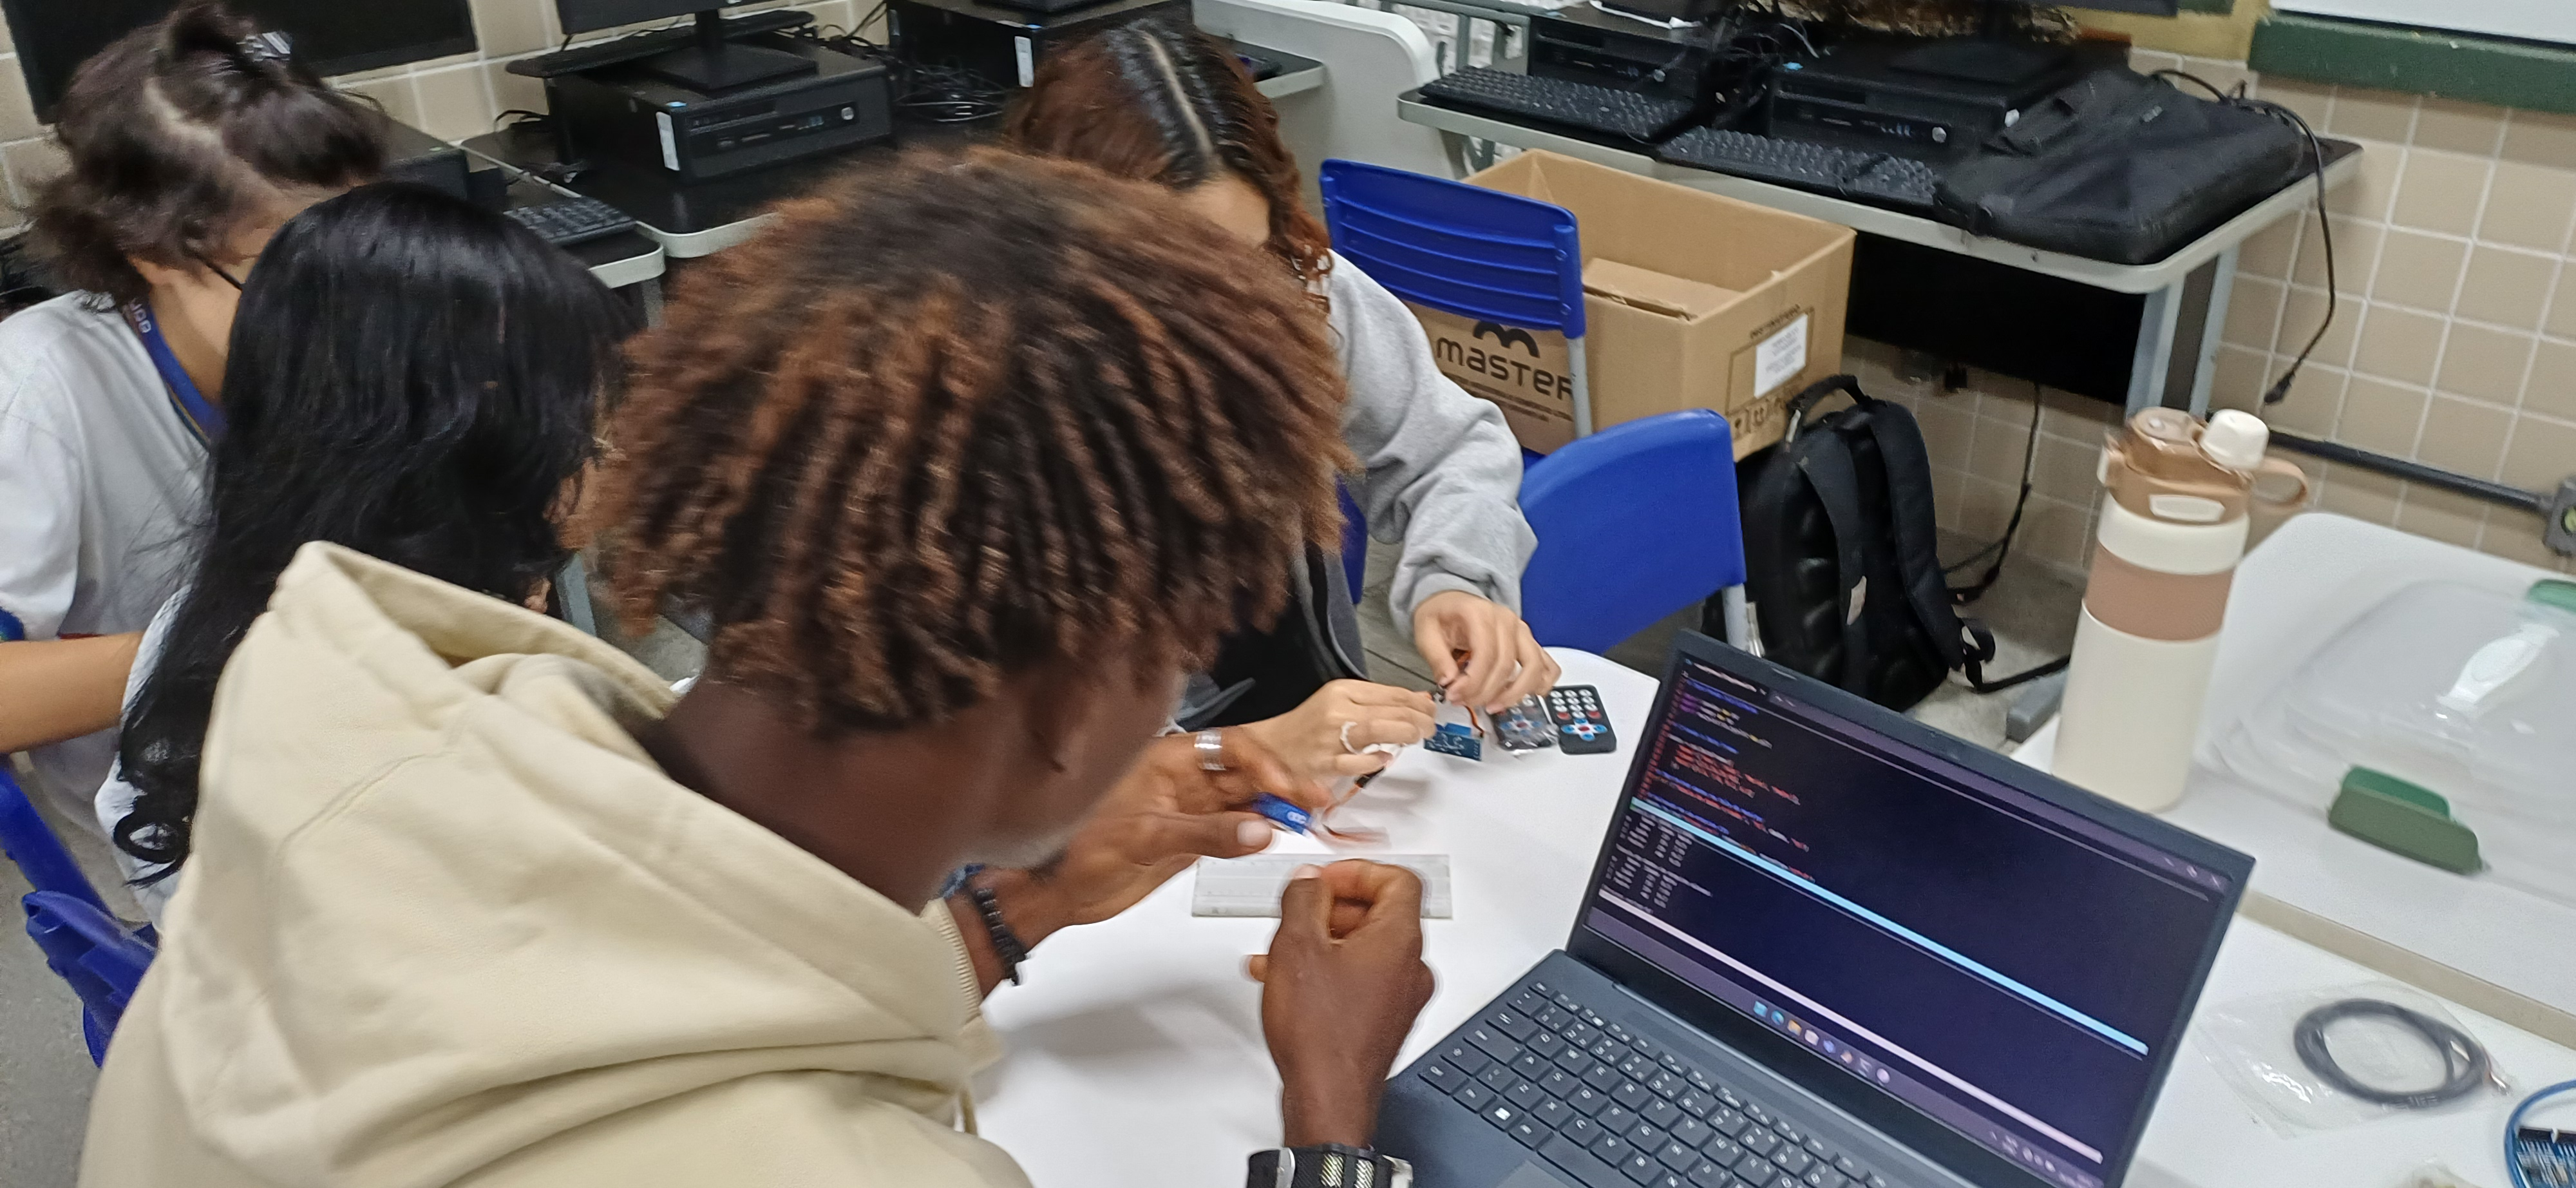
\includegraphics[width=0.4\textwidth]{../Fotos_Projeto_Arduino_Agronegocio/Etapa_4_Construcao/20250926_195233.jpg}
        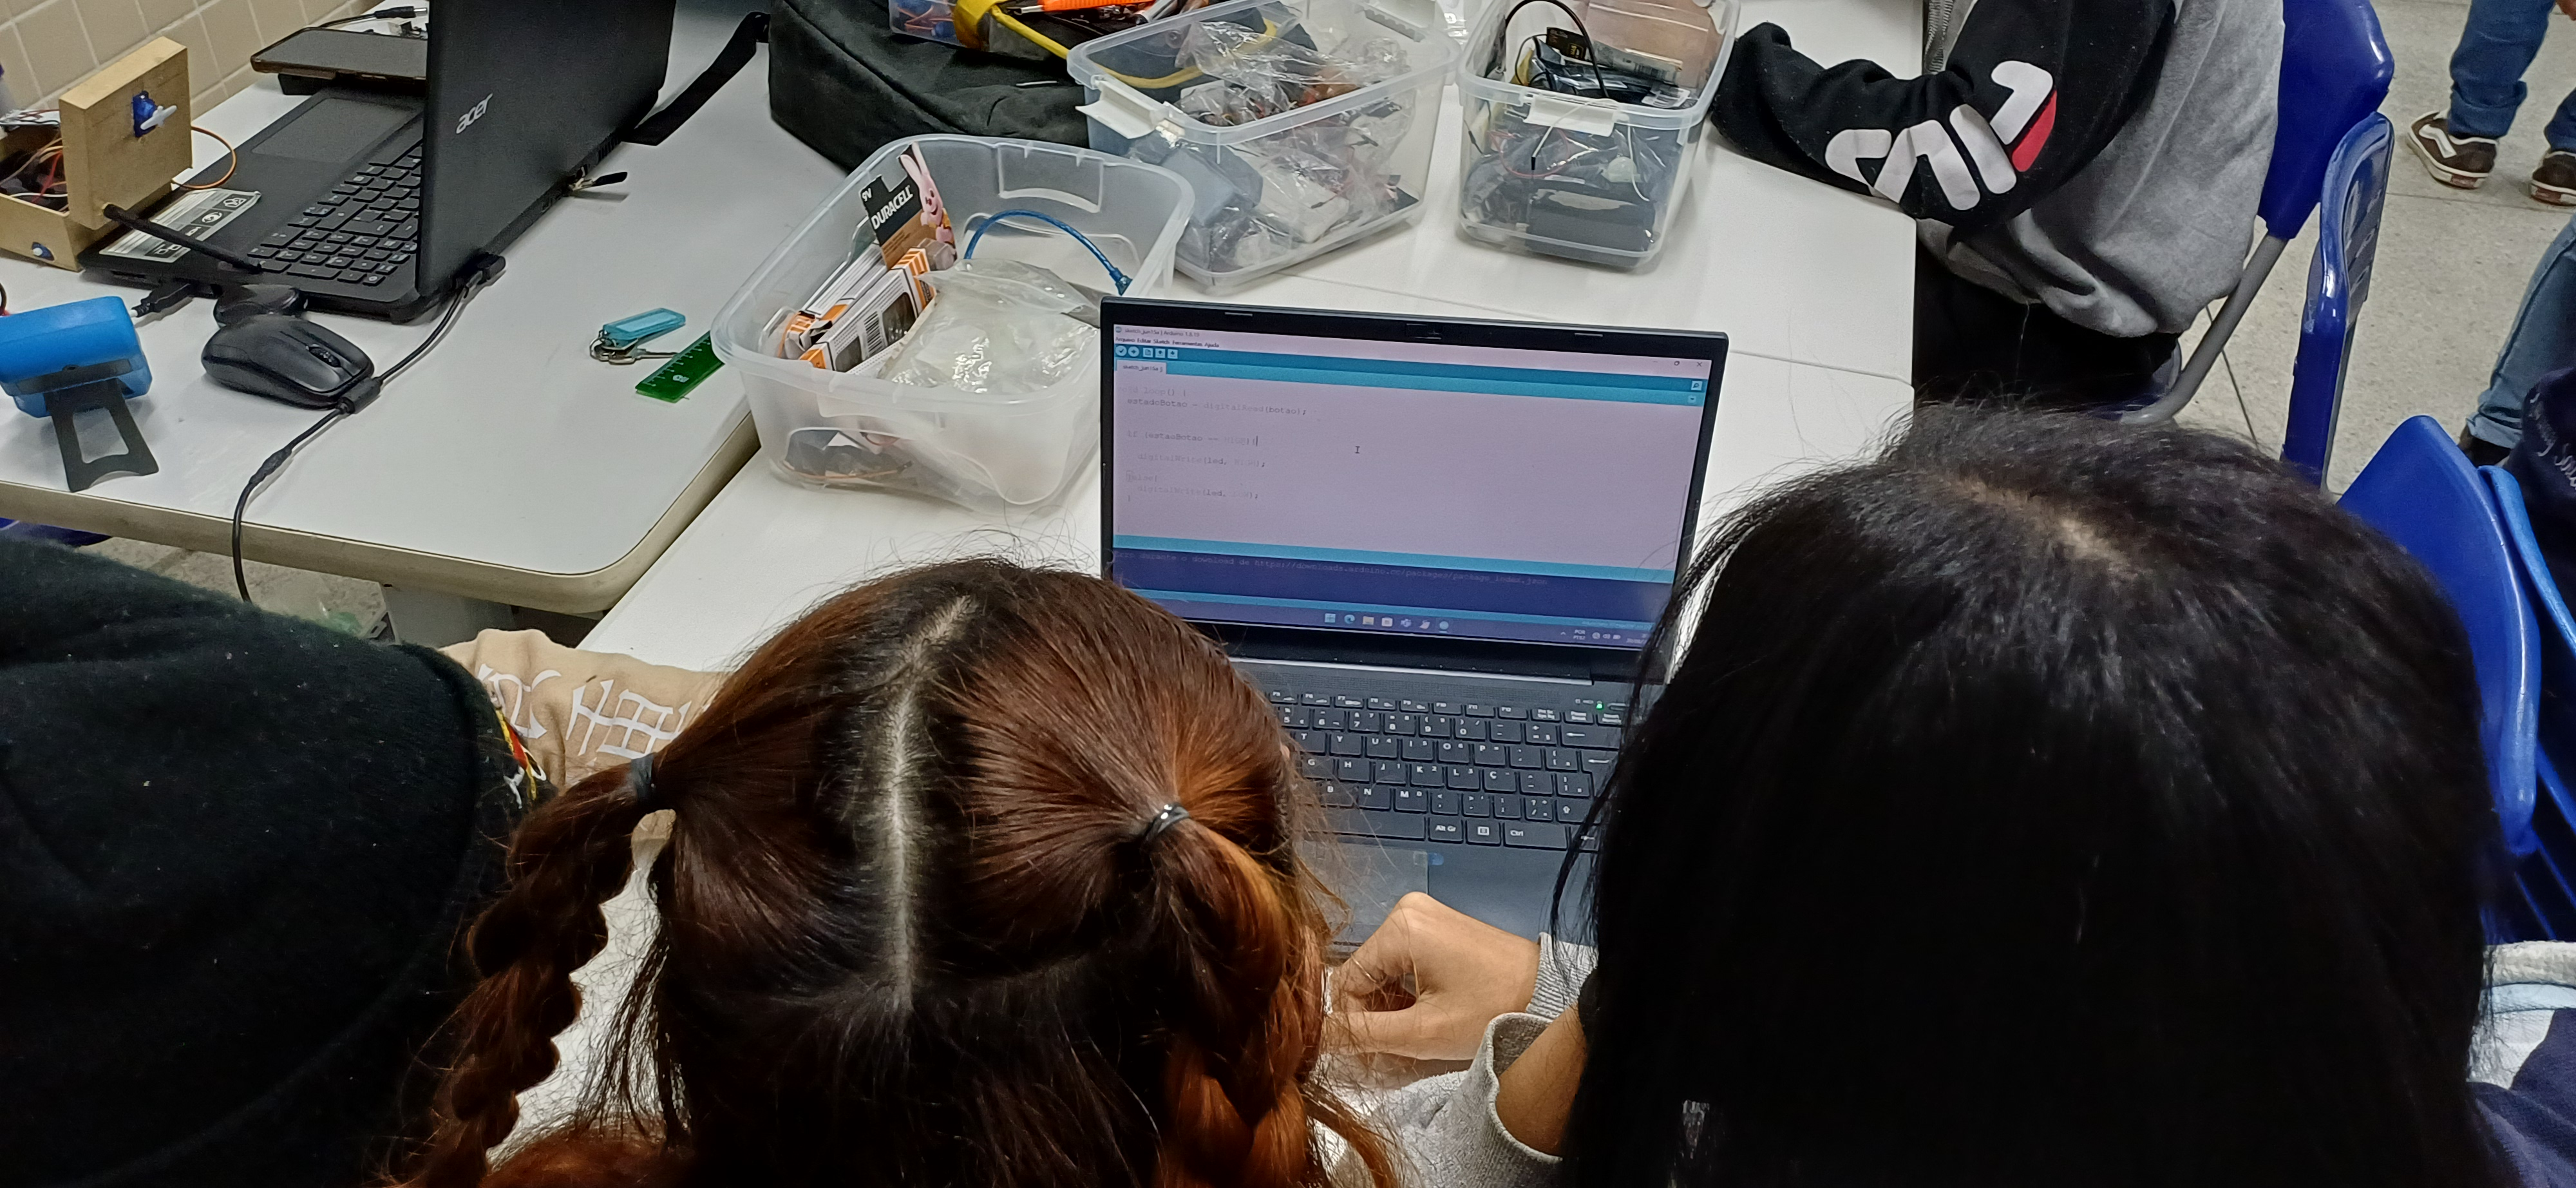
\includegraphics[width=0.4\textwidth]{../Fotos_Projeto_Arduino_Agronegocio/Etapa_3_Condicionais/20250820_203221.jpg}
        \caption{Estudantes desenvolvendo o projeto}
    \end{figure}
\end{frame}

\begin{frame}{Evidências}
    \begin{figure}[h]
        \centering
        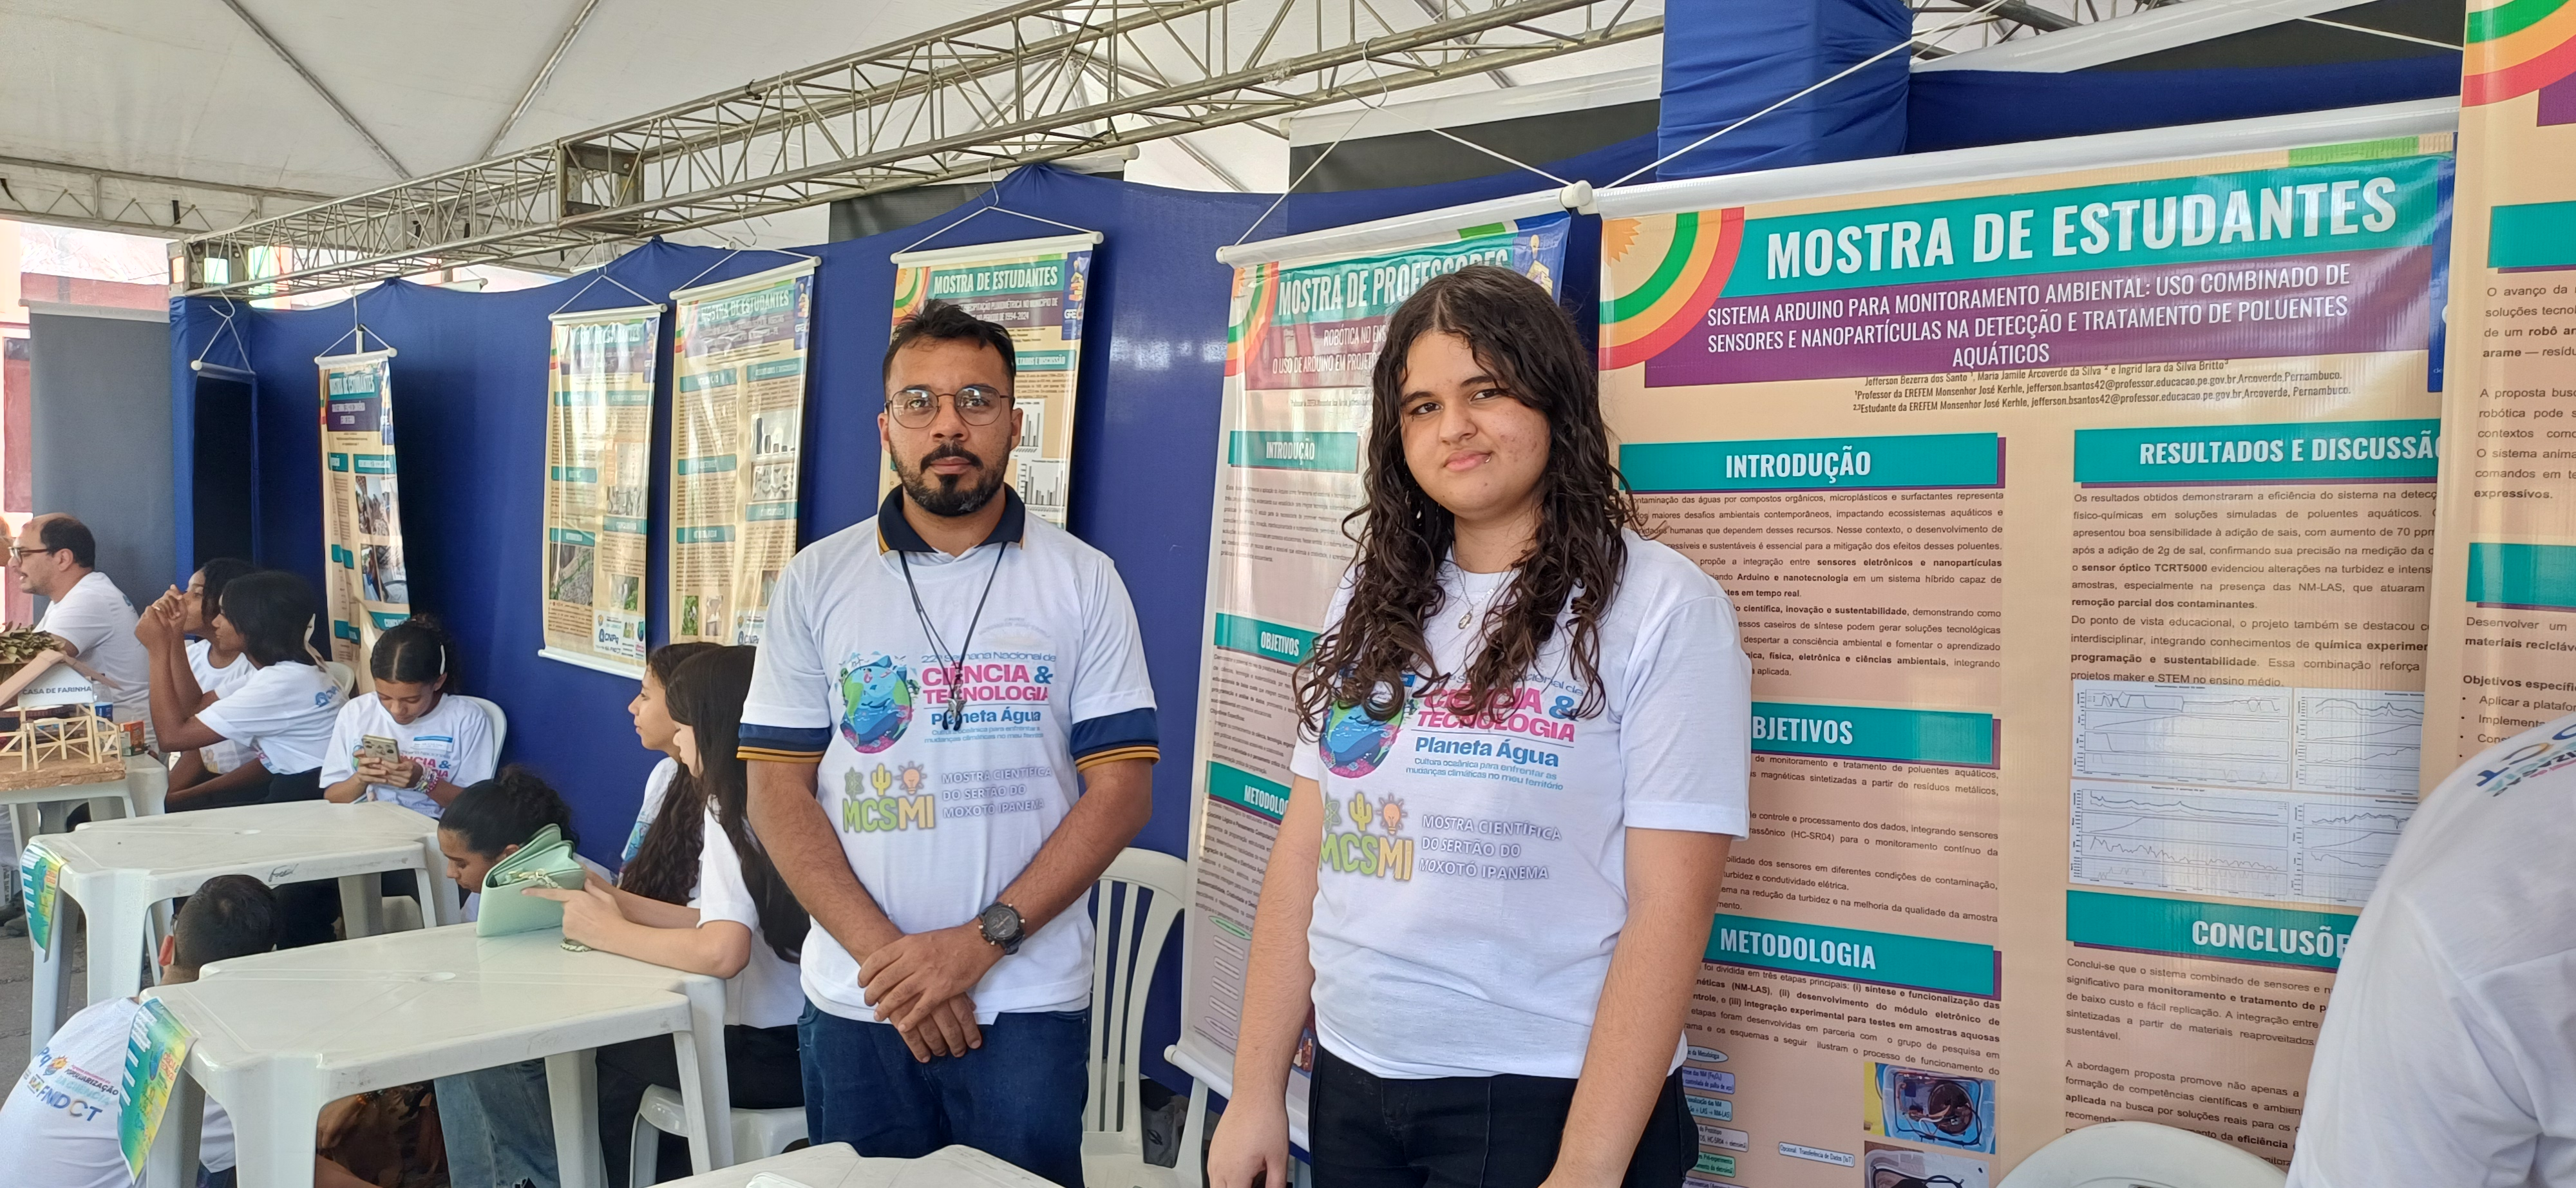
\includegraphics[width=0.4\textwidth]{../Fotos_Projeto_Arduino_Agronegocio/AmostraCientificaMoxoto/AmostraJamile.jpg}
        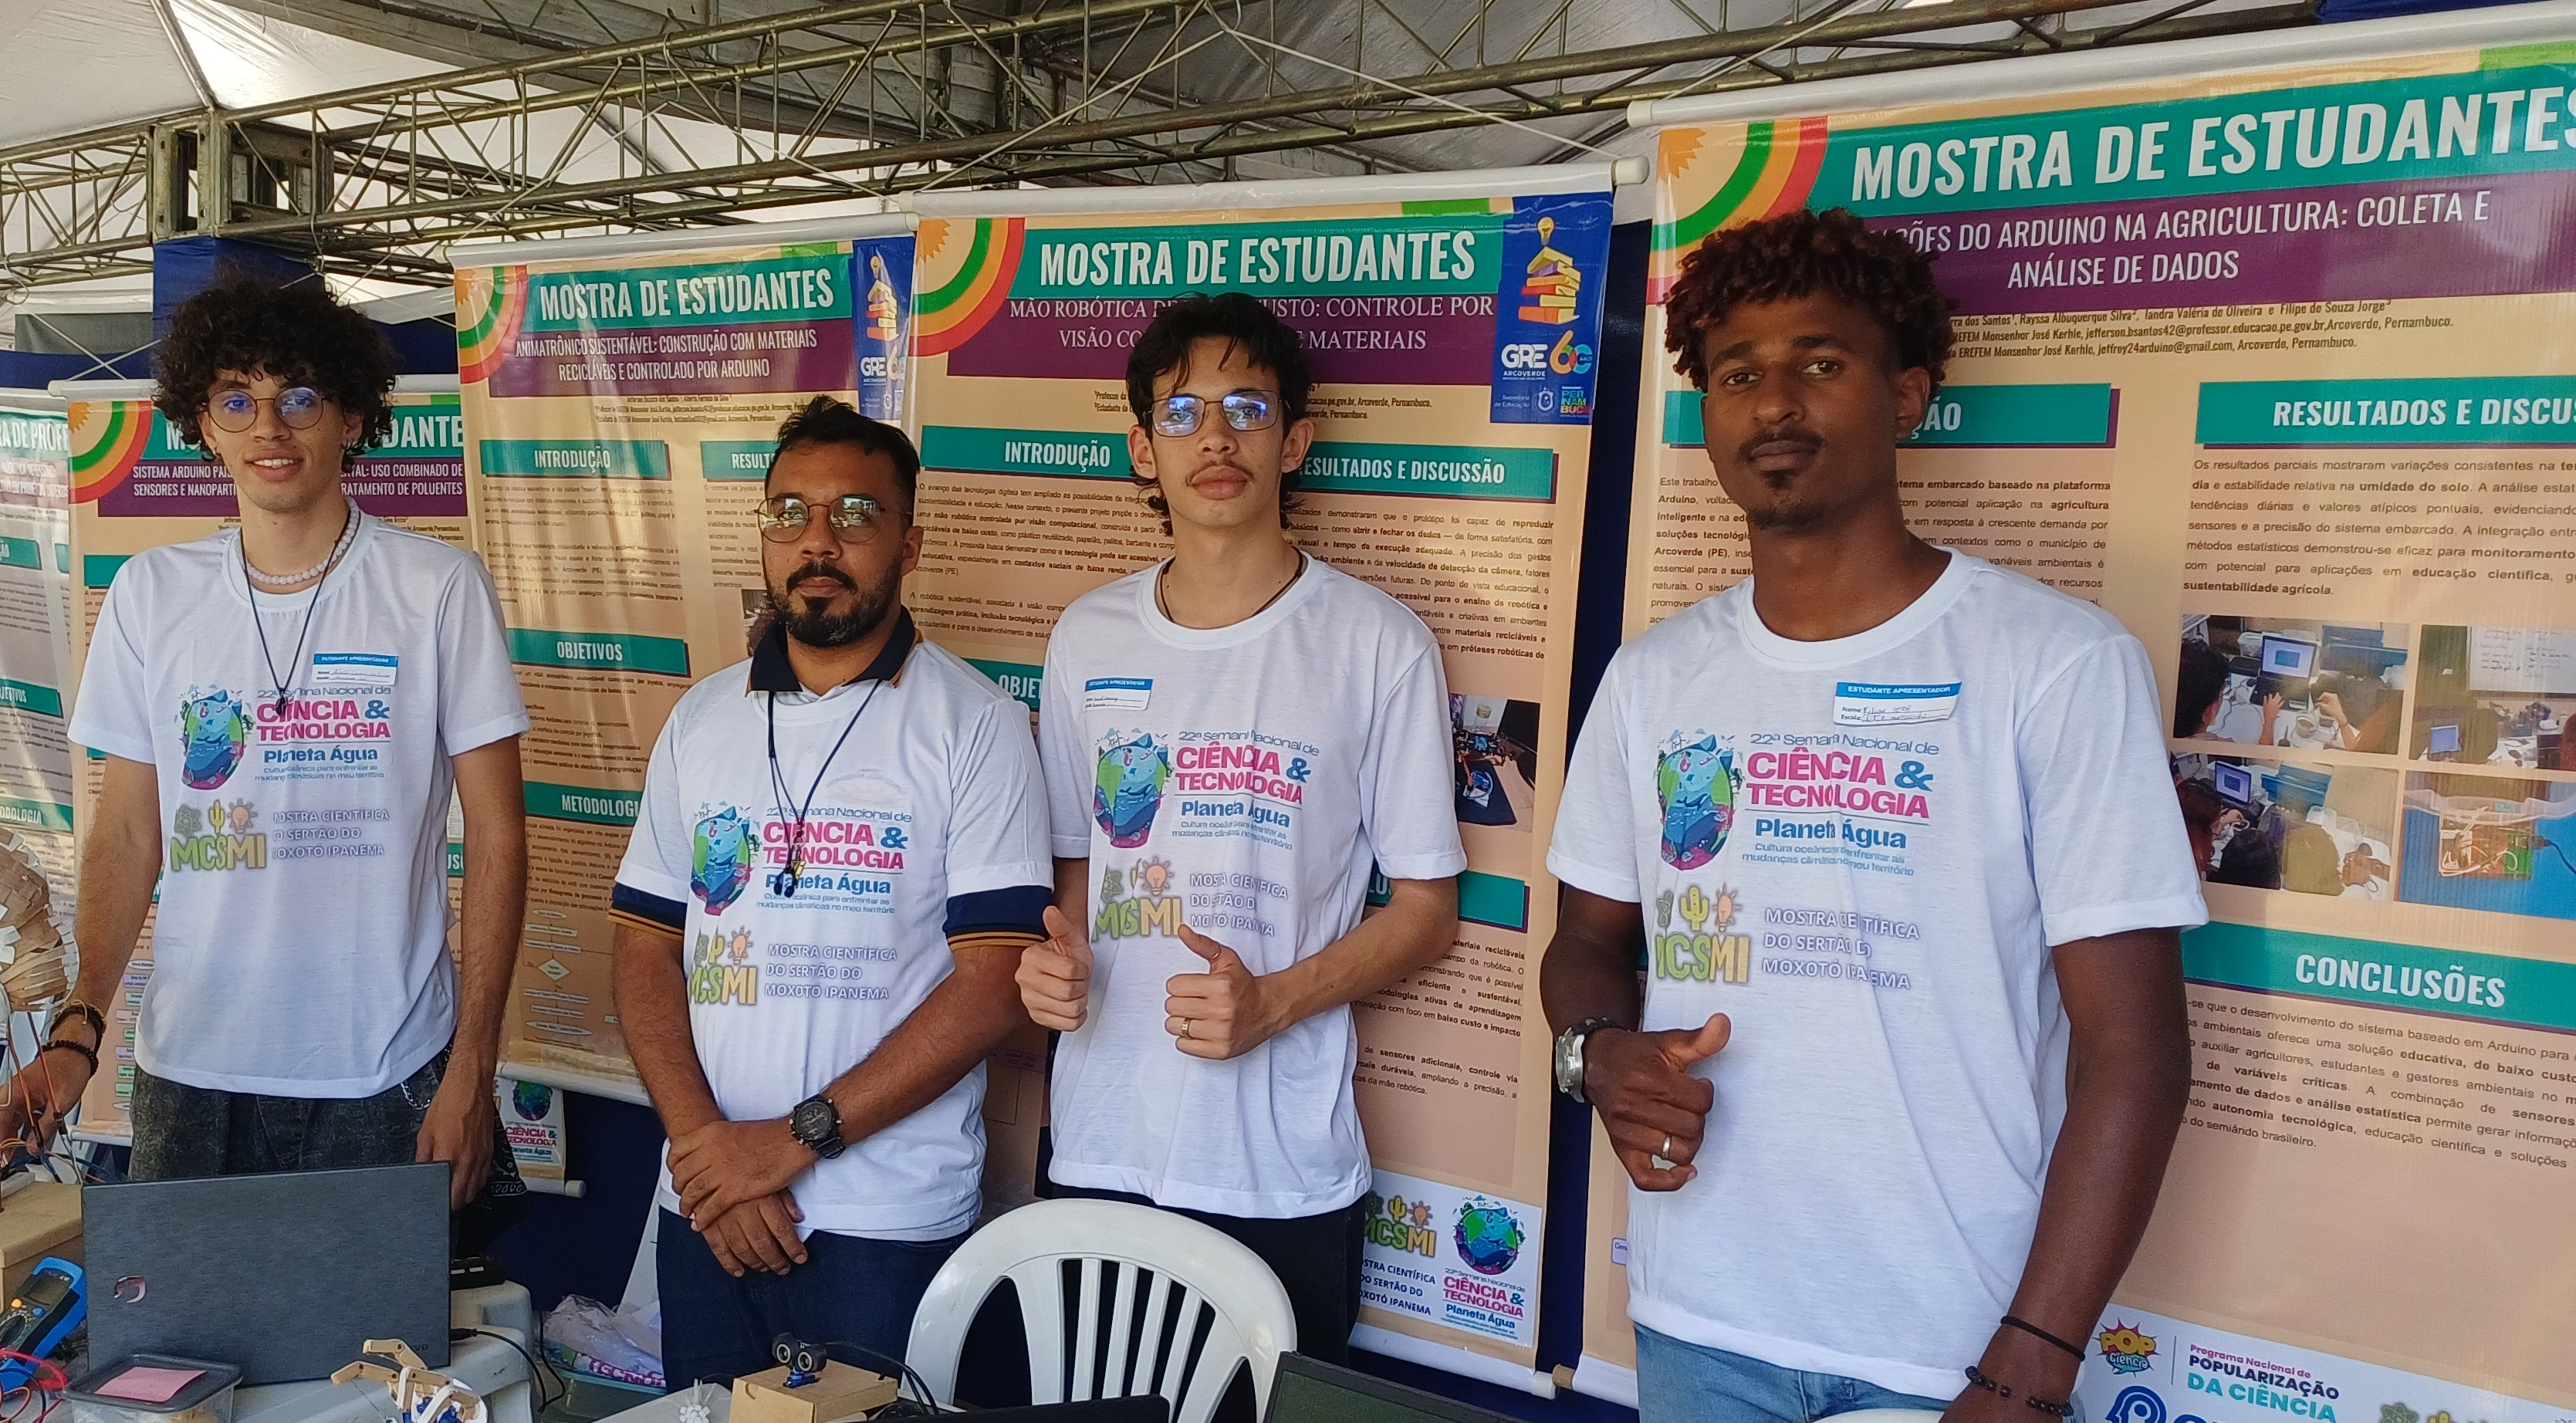
\includegraphics[width=4.8cm, height=2.2cm]{../Fotos_Projeto_Arduino_Agronegocio/AmostraCientificaMoxoto/amostraMeninos.jpg}
        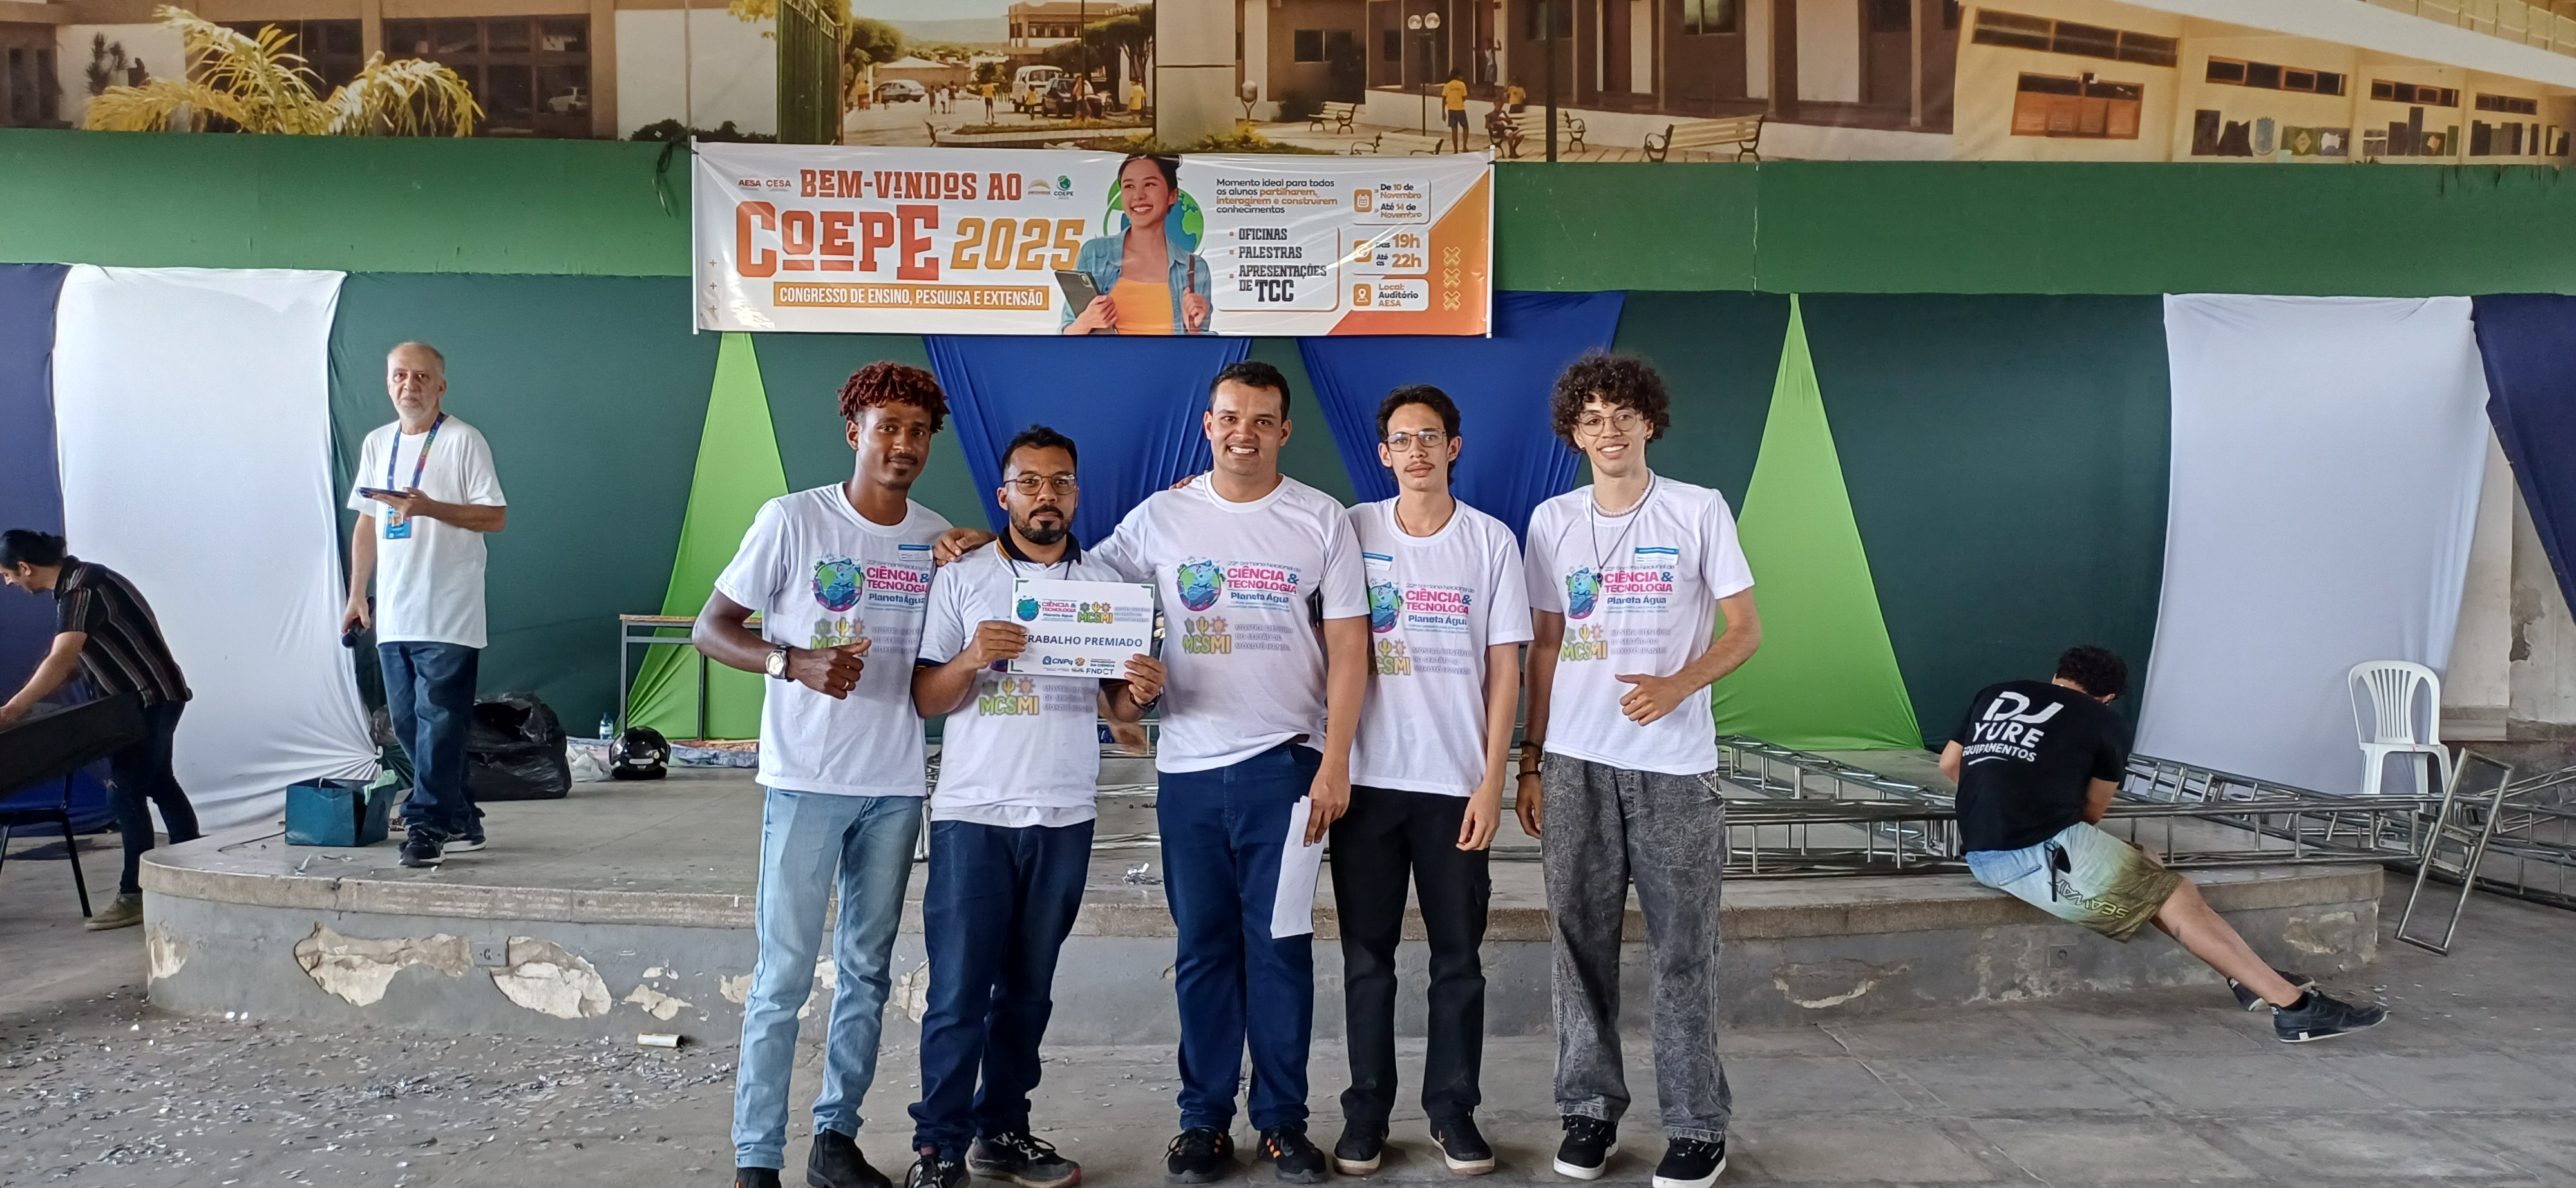
\includegraphics[width=0.4\textwidth]{../Fotos_Projeto_Arduino_Agronegocio/AmostraCientificaMoxoto/AmostraMeninosVencedores.jpg}
        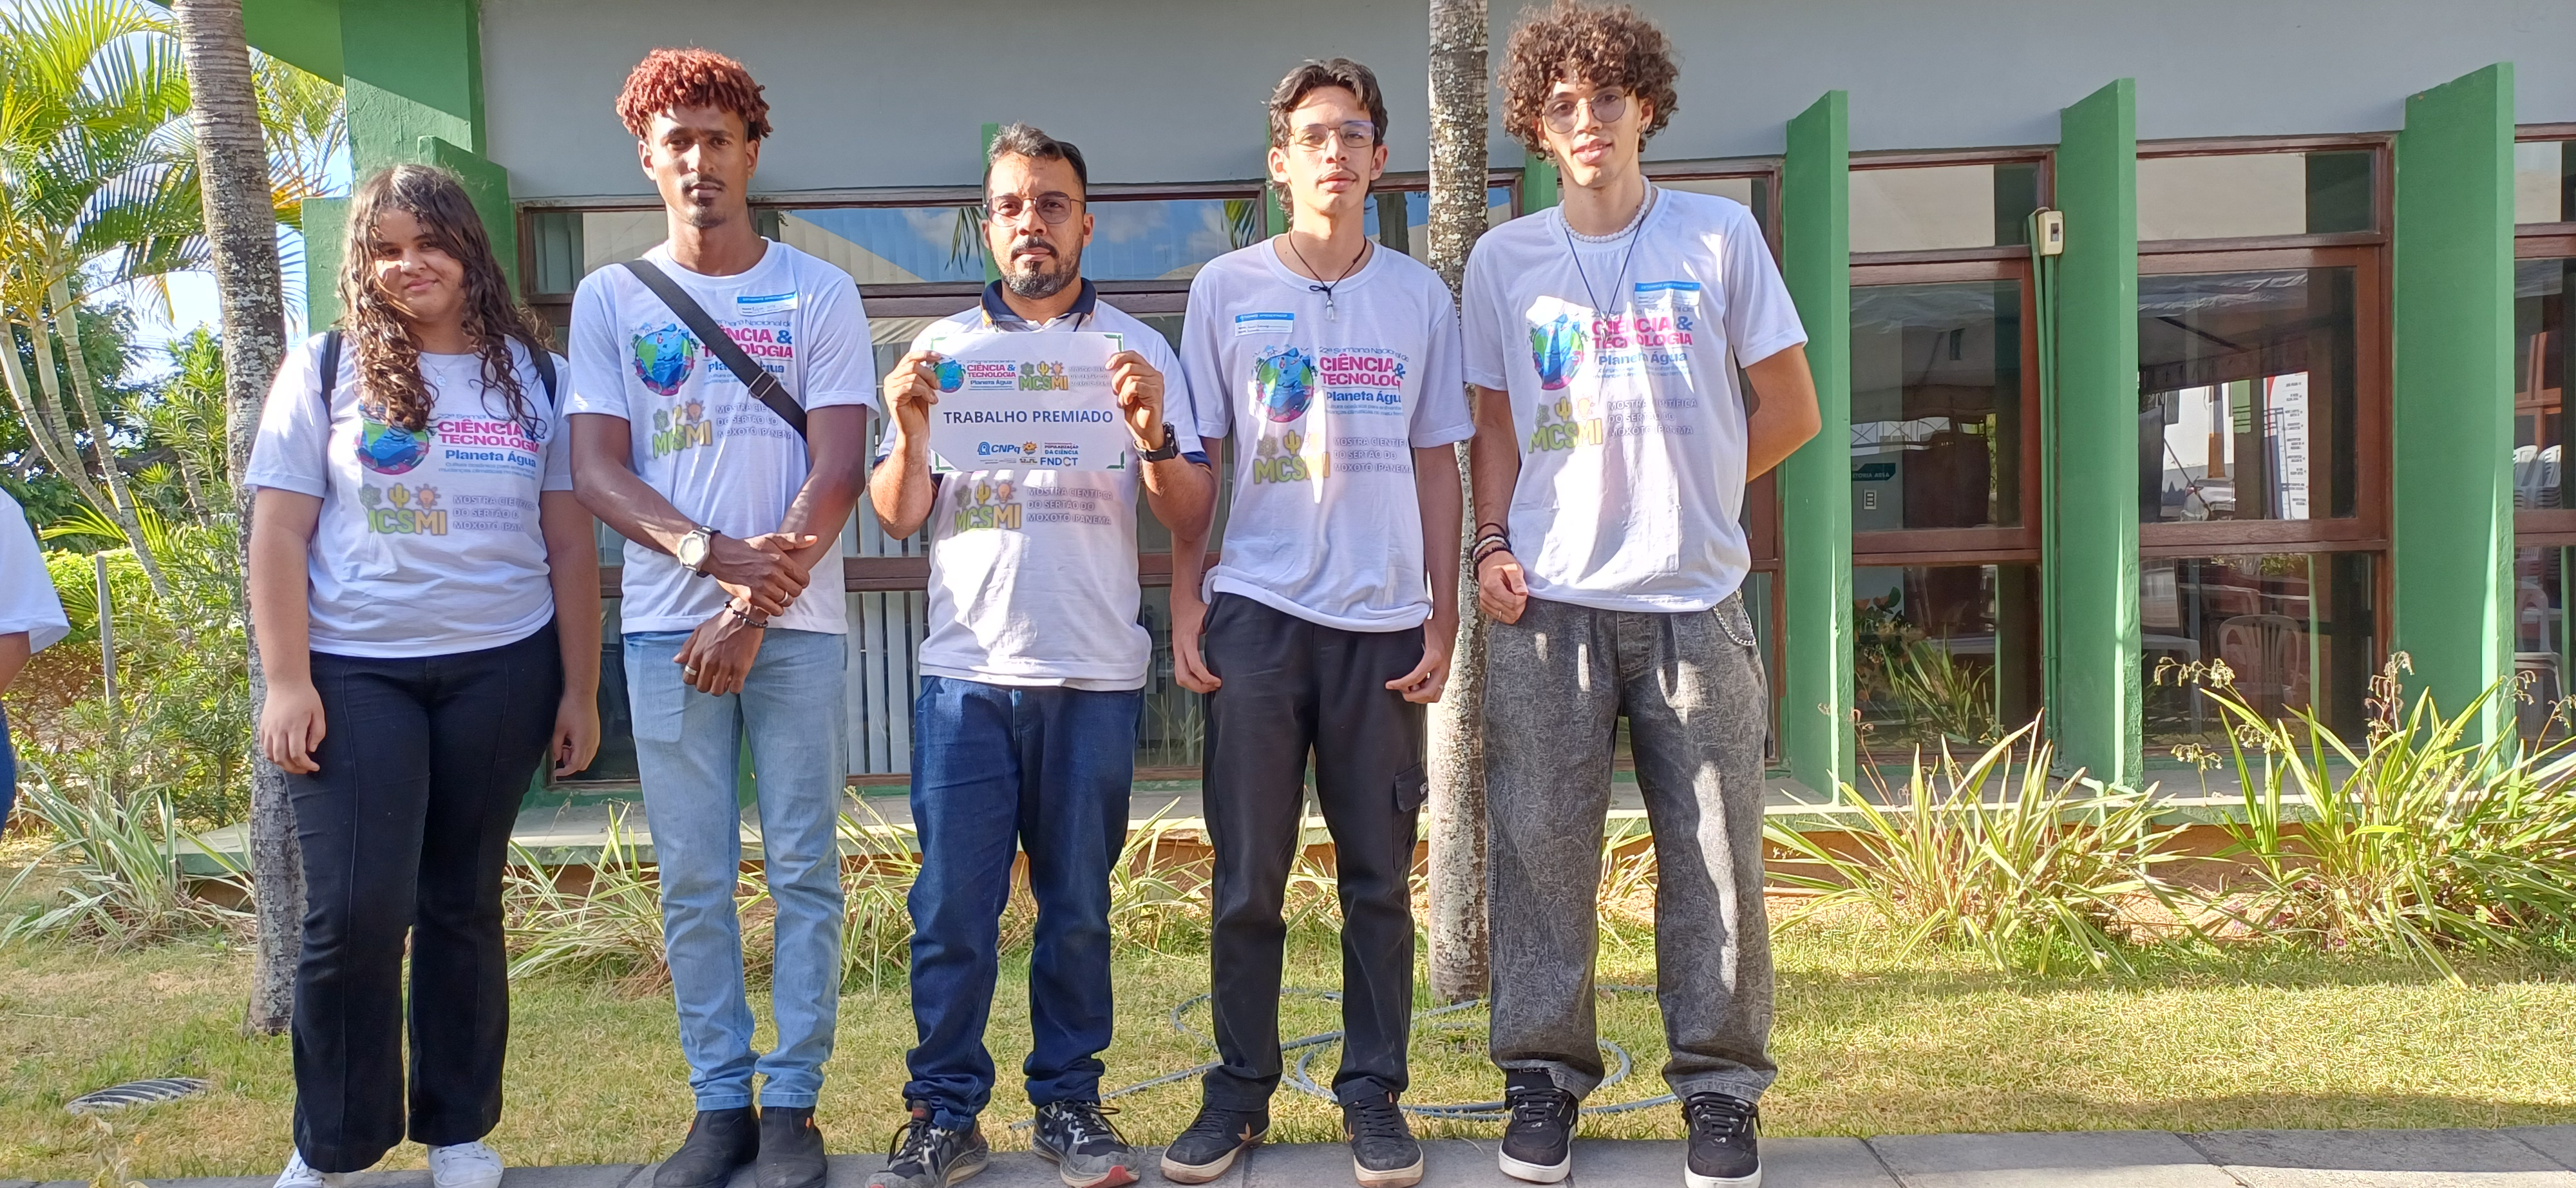
\includegraphics[width=0.4\textwidth]{../Fotos_Projeto_Arduino_Agronegocio/AmostraCientificaMoxoto/AmostraVencedores3.jpg}
        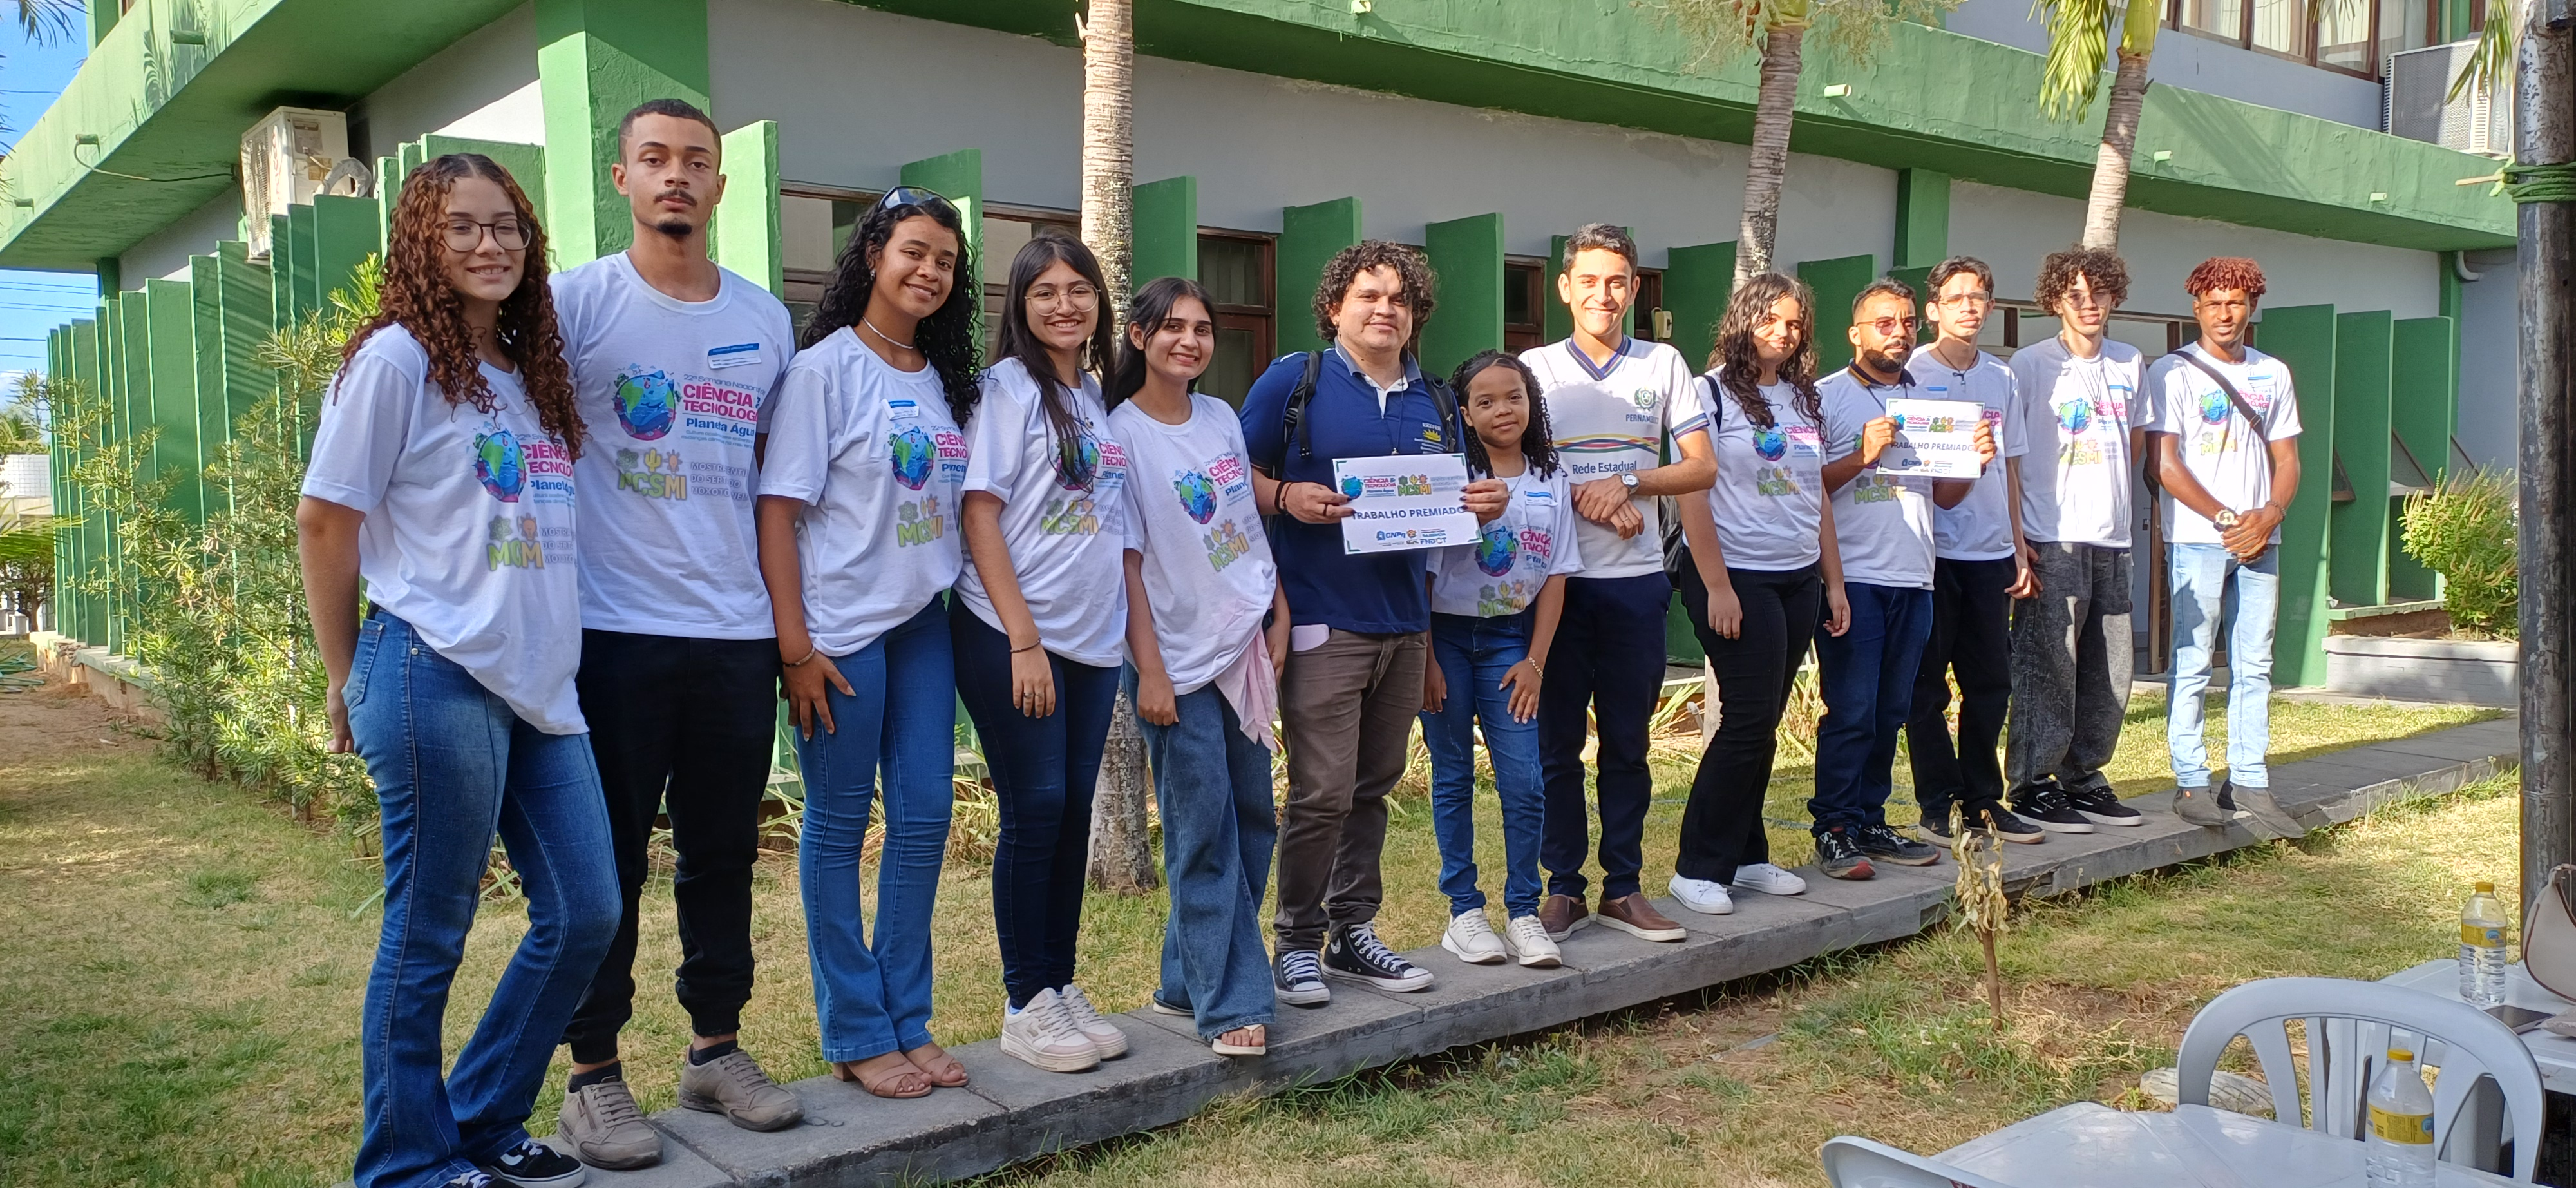
\includegraphics[width=0.4\textwidth]{../Fotos_Projeto_Arduino_Agronegocio/AmostraCientificaMoxoto/AmostraVencedores4.jpg}
        \caption{Estudantes na Amostra Cientifica de Arcoverde}
    \end{figure}
\end{frame}

\begin{frame}{Evidências}
    \begin{figure}[h]
        \centering
        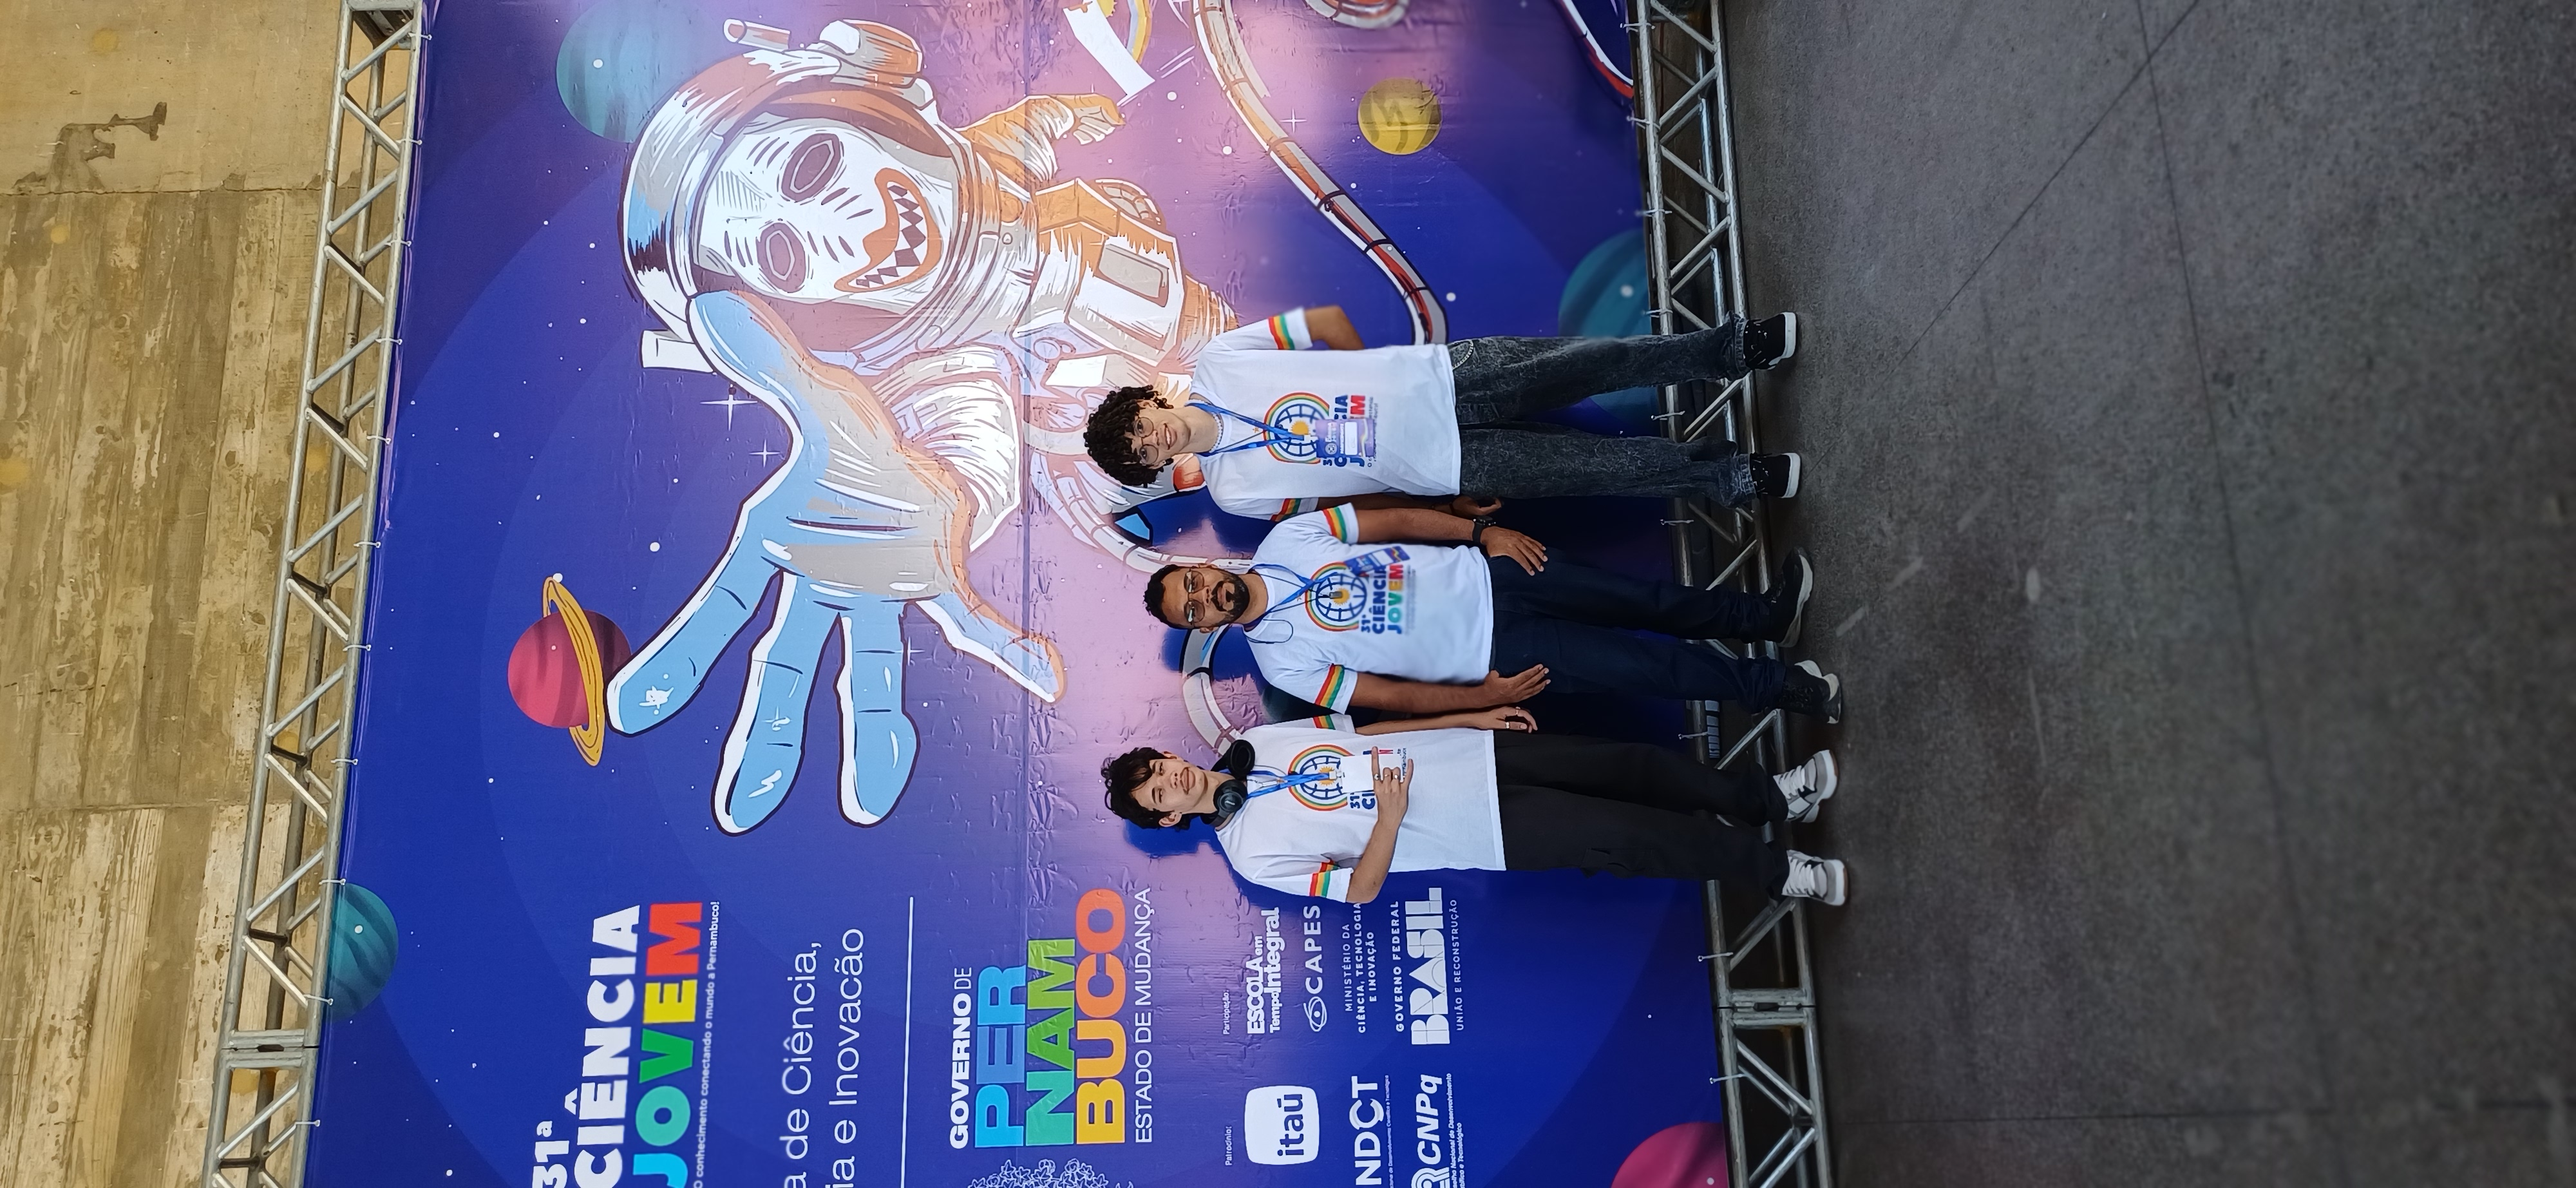
\includegraphics[angle=-90, width=0.25\textwidth]{../Fotos_Projeto_Arduino_Agronegocio/CienciaJovem/CienciaJovem1.jpg}
        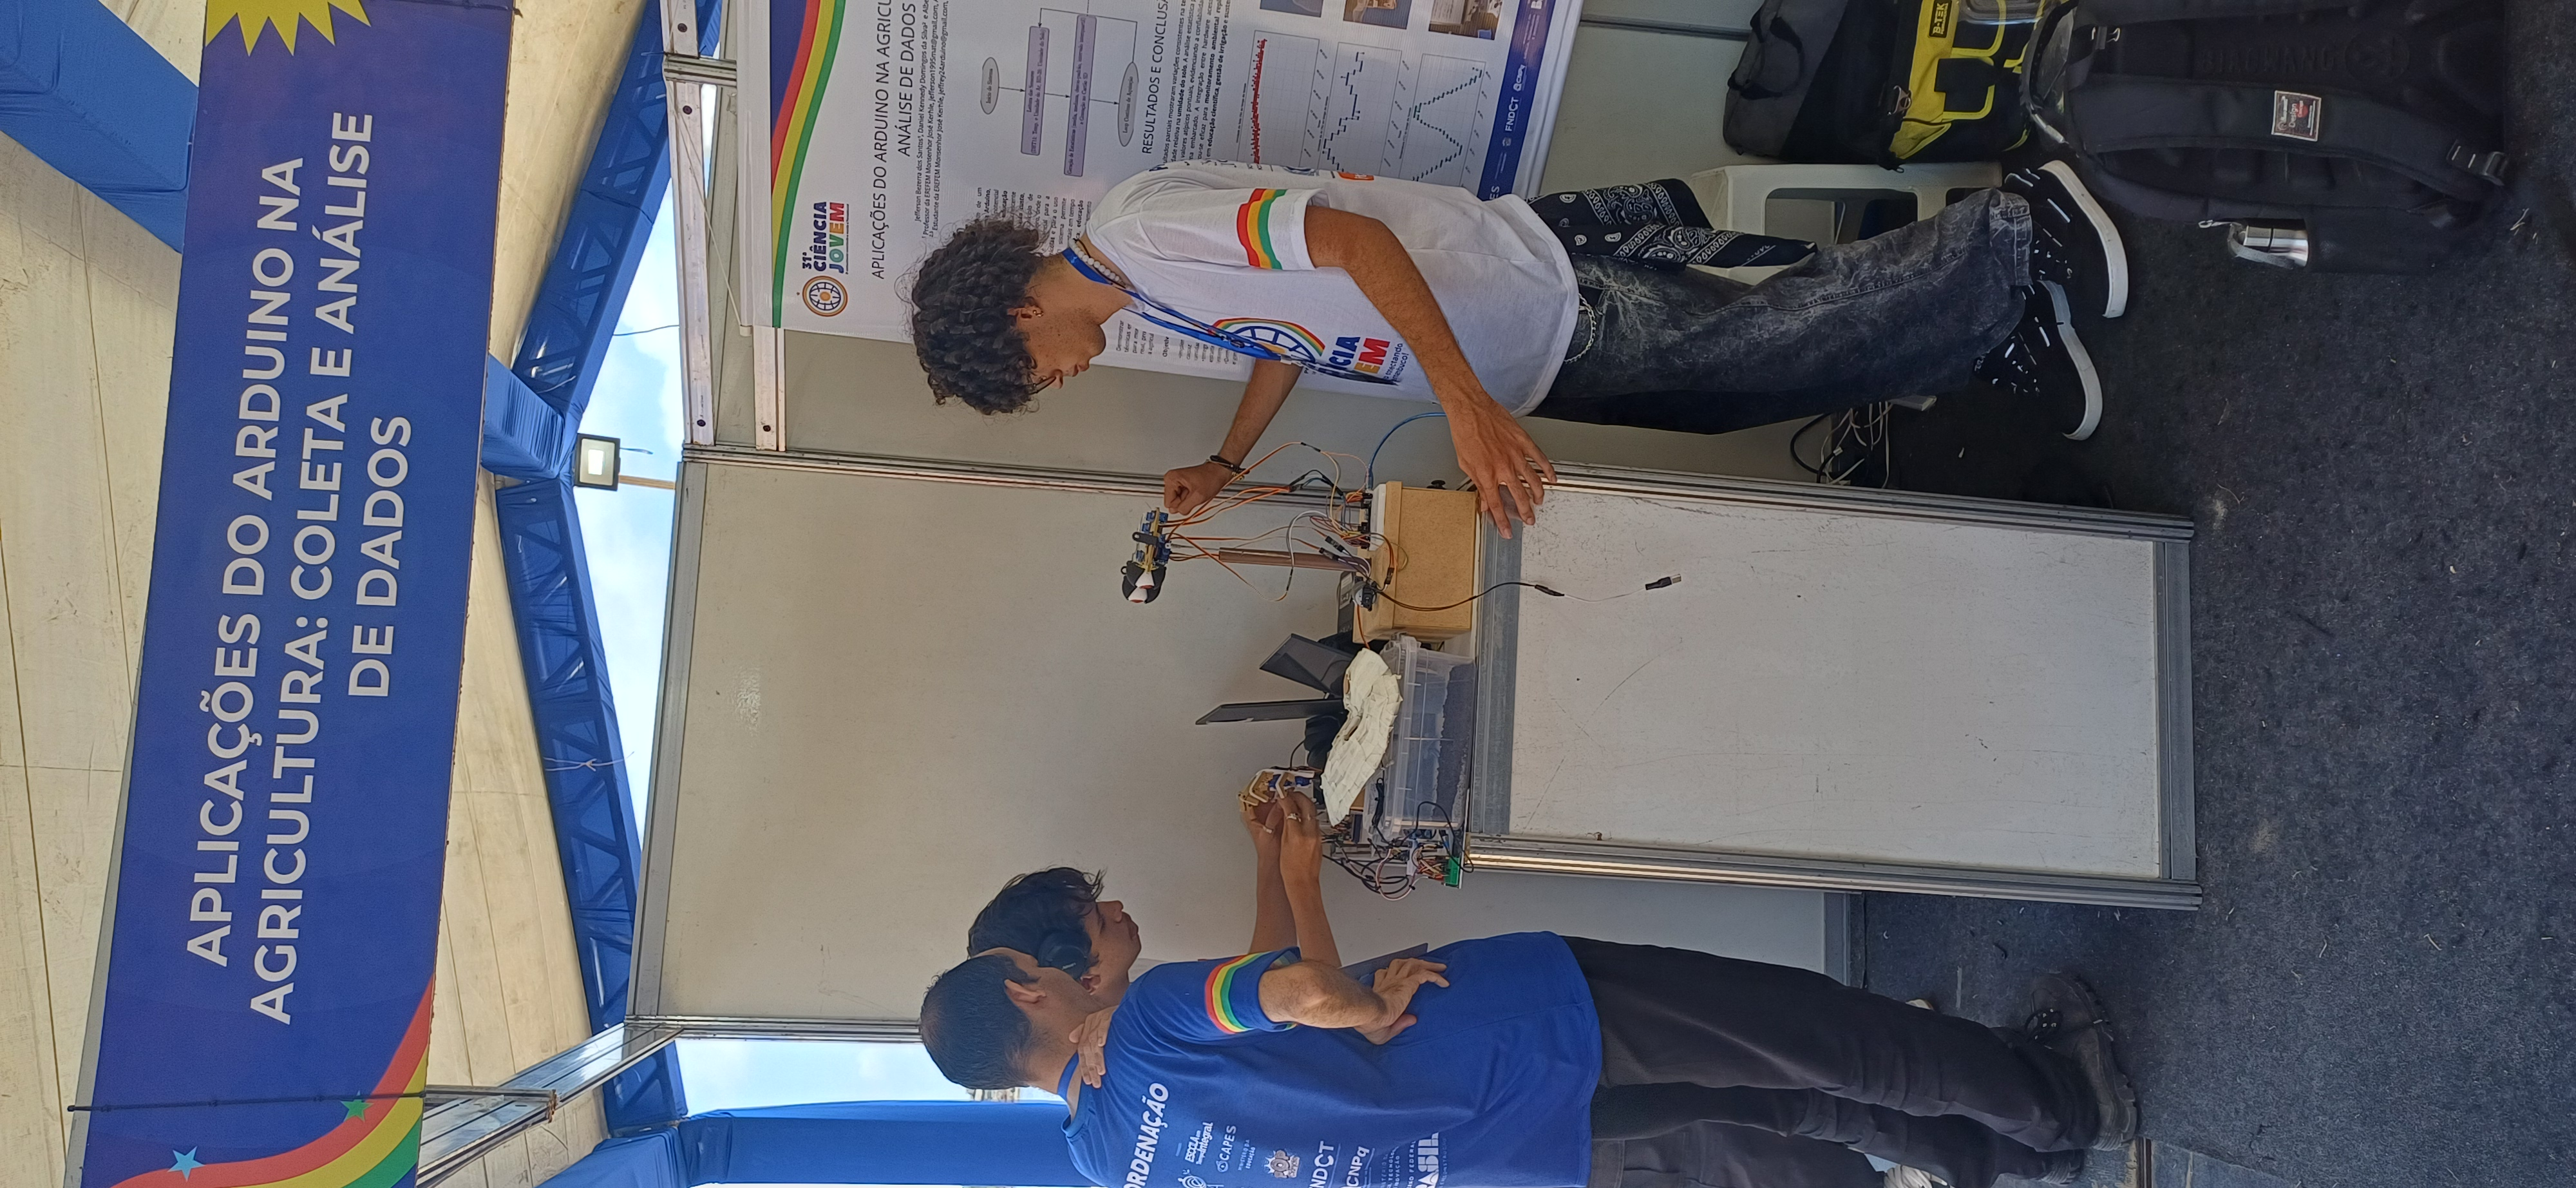
\includegraphics[angle=-90, width=0.25\textwidth]{../Fotos_Projeto_Arduino_Agronegocio/CienciaJovem/CienciaJovem5.jpg}
        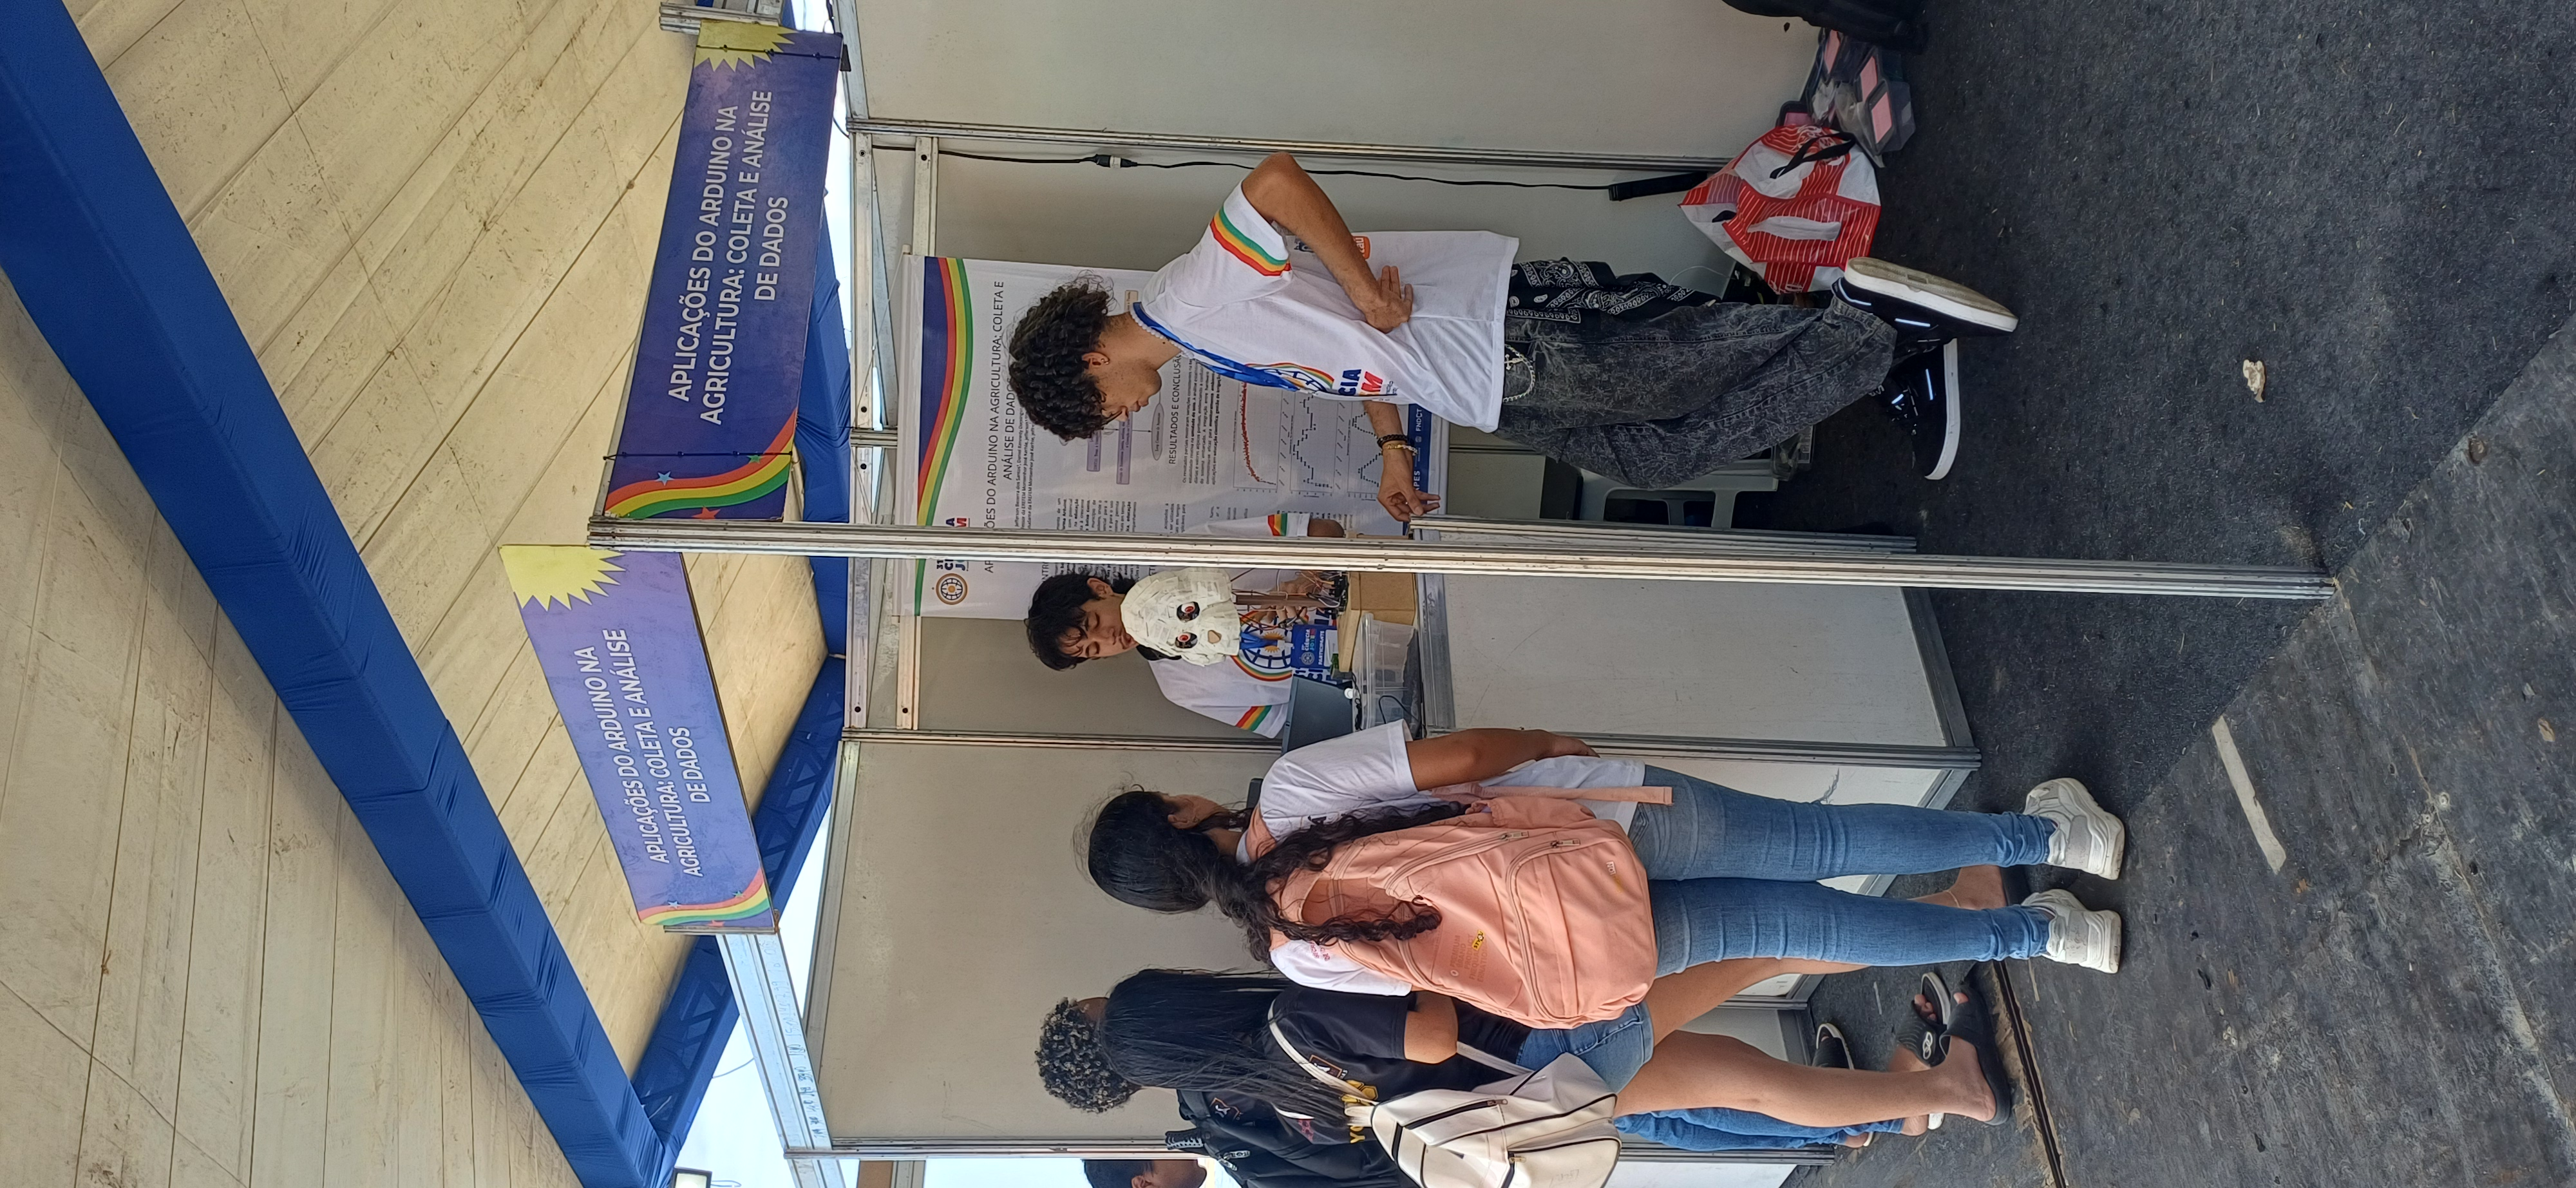
\includegraphics[angle=-90, width=0.25\textwidth]{../Fotos_Projeto_Arduino_Agronegocio/CienciaJovem/CienciaJovem4.jpg}
        \caption{Estudantes no Ciência Jovem}
    \end{figure}
\end{frame}

% ==========================================================
% ==================== INDICADORES QUANTITATIVOS ===========
% ==========================================================

\section{Indicadores}
\begin{frame}{Indicadores Quantitativos}
\begin{itemize}
    \item \textbf{Bolsistas contemplados:} 10 estudantes
    \item \textbf{Produtos desenvolvidos:} Analizador de solo (sistema arduino + python)
    \item \textbf{Pessoas impactadas/beneficiadas:} Estudantes e comunidade 
\end{itemize}
\end{frame}


% ==========================================================
% ==================== EXPECTATIVAS =======================
% ==========================================================

\section{Expectativas}
\begin{frame}{Expectativas e Próximos Passos}
\begin{itemize}
    \item Expandir o número de áreas monitoradas.
    \item Incorporar sensores adicionais (luminosidade, pH do solo).
    \item Teste com diferentes amostras de diferente tipos de solo.
    \item Desenvolver aplicativo de monitoramento remoto em tempo real.
\end{itemize}
\end{frame}

% ==========================================================
% ==================== CONCLUSÃO ==========================
% ==========================================================

\section{Conclusão}
\begin{frame}{Conclusão}
\begin{itemize}
    \item Sistema de baixo custo eficaz e acessível.
    \item Integração entre eletrônica, estatística e práticas agrícolas.
    \item Potencial produtivo elevado com baixo risco climático.
\end{itemize}
\end{frame}

\begin{frame}
    \centering

    {\Large \textbf{Obrigado!!!}}\\[0.8cm]

    % Área com QR + título (título aparece só acima do QR)
    \begin{minipage}{0.32\textwidth}
        \centering
        {\small \textbf{Referências e Documentação}}\\[0.1cm]
        
\includegraphics[width=\linewidth]{qrGrupoPesquisa.png}
    \end{minipage}
    \hspace{0.6cm}
    % Área com logo FACEPE (sem título)
    \begin{minipage}{0.4\textwidth}
        \centering
        
\includegraphics[width=\linewidth]{facepe.png}
    \end{minipage}

    \\[1cm]

    {\textbf{\inserttitle}}\\[0.5cm]
    {\insertauthor}\\[0.3cm]
    {\small \insertdate}
\end{frame}

\end{document}

